%
%#############################################
\ifFIGS
\begin{table}[t]\centering

  \mnp{\textwidth}{
\captionN{Out-performance of \enet recommendations over WHO 
for Influenza A vaccine composition}\label{tabperf}\centering
\vspace{-10pt}

\sffamily\fontsize{7}{8}\selectfont

\begin{tabular}{C{.5in}|C{.35in}|C{.7in}|C{0.35in}|C{0.35in}|C{0.4in}|C{0.35in}|C{0.35in}|C{0.4in}|C{0.35in}|C{0.35in}|C{0.4in}}
\multicolumn{3}{c}{}&\multicolumn{3}{c}{Two decades}&\multicolumn{3}{|c}{One decade}&\multicolumn{3}{|c}{2015-2019}\\\hline
Subtype & Gene & Hemisphere & WHO Error & \qnet Error & Improvement (\%) & WHO Error & \qnet Error & Improvement (\%) & WHO Error & \qnet Error &  Improvement (\%)\\\hline
H1N1&HA& North &12.67&8.76&30.83&4.38&1.19&72.83&2.52&0.33&86.79\\\hline
H1N1&HA& South &13.57&9.00&33.68&4.67&1.62&65.31&2.52&0.62&75.47\\\hline
\rowcolor{lightgray}H1N1&HA&Average&13.12&8.88&32.25&4.53&1.40&69.07&2.52&0.48&81.13\\\hline
H3N2&HA& North &7.65&4.71&38.46&5.00&2.94&41.18&1.82&0.88&51.61\\\hline
H3N2&HA& South &7.59&4.82&36.43&4.94&3.00&39.29&1.82&0.94&48.39\\\hline
\rowcolor{lightgray}H3N2&HA&Average&7.62&4.77&37.44&4.97&2.97&40.24&1.82&0.91&50.00\\\hline
H1N1&NA& North &8.29&6.90&16.67&2.62&1.10&58.18&2.10&0.48&77.27\\\hline
H1N1&NA& South &9.14&8.38&8.33&3.00&1.43&52.38&2.10&0.76&63.64\\\hline
\rowcolor{lightgray}H1N1&NA&Average&8.72&7.64&12.50&2.81&1.27&55.28&2.10&0.62&70.46\\\hline
H3N2&NA& North &4.21&3.63&13.75&2.11&1.79&15.00&1.32&0.32&76.00\\\hline
H3N2&NA& South &4.68&4.16&11.24&2.58&2.05&20.41&1.32&0.42&68.00\\\hline
\rowcolor{lightgray}H3N2&NA&Average&4.44&3.90&12.50&2.34&1.92&17.70&1.32&0.37&72.00\\\hline
\end{tabular}

% \end{table*}
% \else
% \refstepcounter{table}\label{tabperf}
% \fi
% %#############################################
% %#############################################


% %#############################################
% %#############################################
% \begin{table}[!hb]\centering
}
\vskip .5em

  \mnp{\textwidth}{
\captionN{H1N1 HA Northern Hemisphere}\label{tabrec0}
\vspace{-10pt}

\sffamily\fontsize{7}{8}\selectfont

\begin{tabular}{L{.37in}|L{1.62in}|L{1.62in}|L{1.62in}|L{.25in}|L{.25in}}\hline
Year & WHO Recommendation & Dominant Strain & \qnet Recommendation & WHO Error & \qnet Error \\\hline
2001-02& A/New  Caledonia/20/99 & A/Canterbury/41/2001 & A/Dunedin/2/2000 &4&6\\\hline
2002-03& A/New  Caledonia/20/99 & A/Taiwan/567/2002 & A/New  York/241/2001 &3&1\\\hline
2003-04& A/New  Caledonia/20/99 & A/Memphis/5/2003 & A/New  York/291/2002 &5&2\\\hline
2004-05& A/New  Caledonia/20/99 & A/Thailand/Siriraj-Rama-TT/2004 & A/New  York/222/2003 &7&4\\\hline
2005-06& A/New  Caledonia/20/99 & A/Niedersachsen/217/2005 & A/Canterbury/106/2004 &8&10\\\hline
2006-07& A/New  Caledonia/20/99 & A/India/34980/2006 & A/Auckland/619/2005 &6&1\\\hline
2007-08& A/Solomon  Islands/3/2006 &A/Norway/1701/2007& A/New  York/8/2006 &8&11\\\hline
2008-09& A/Brisbane/59/2007 & A/Pennsylvania/02/2008 & A/Kentucky/UR06-0476/2007 &2&2\\\hline
2009-10& A/Brisbane/59/2007 & A/Singapore/ON1060/2009 & A/Hong  Kong/549/2008 &119&119\\\hline
2010-11& A/California/7/2009 & A/England/01220740/2010 & A/New  York/14/2009 &5&1\\\hline
2011-12& A/California/7/2009 & A/Punjab/041/2011 & A/Kansas/01/2010 &7&2\\\hline
2012-13& A/California/7/2009 & A/British  Columbia/001/2012 &A/Moscow/WRAIR4308T/2011&11&4\\\hline
2013-14& A/California/7/2009 &A/Moscow/CRIE-32/2013& A/Helsinki/1199/2012 &10&2\\\hline
2014-15& A/California/7/2009 & A/Thailand/CU-C5169/2014 & A/Maryland/02/2013 &12&0\\\hline
2015-16& A/California/7/2009 & A/Georgia/15/2015 & A/Utah/3691/2014 &14&2\\\hline
2016-17& A/California/7/2009 & A/Hawaii/21/2016 & A/Adana/08/2015 &16&0\\\hline
2017-18& A/Michigan/45/2015 & A/Michigan/291/2017 & A/Beijing-Huairou/SWL1335/2016 &5&4\\\hline
2018-19& A/Michigan/45/2015 & A/Washington/55/2018 & A/India/C1721549/2017 &6&1\\\hline
2019-20& A/Brisbane/02/2018 & A/Kentucky/06/2019 & A/New  Jersey/01/2018 &5&1\\\hline
2020-21& A/Hawaii/70/2019 &A/Togo/905/2020& A/Italy/8949/2019 &4&8\\\hline
2021-22& A/Victoria/2570/2019 &A/Ireland/20935/2022& A/Togo/45/2021 &9&3\\\hline
2022-23& -1 &-1& A/Netherlands/00068/2022 &-1&-1\\\hline
\end{tabular}

\flushleft

\fontsize{7}{7}\selectfont
$^\star$ Dominant strain is calculated as the one closest to the centroid in the strain space that year in the edit distance metric

% \end{table}

% %#############################################
% %#############################################

% \begin{table}[!hb]\centering
}
\vskip .5em
\mnp{\textwidth}{
  
\captionN{H1N1 HA Southern Hemisphere}\label{tabrec1}

\sffamily\fontsize{7}{8}\selectfont

\begin{tabular}{L{.37in}|L{1.62in}|L{1.62in}|L{1.62in}|L{.25in}|L{.25in}}\hline
Year & WHO Recommendation & Dominant Strain & \qnet Recommendation & WHO Error & \qnet Error \\\hline
2001-02& A/New  Caledonia/20/99 & A/Canterbury/41/2001 & A/South  Canterbury/50/2000 &4&6\\\hline
2002-03& A/New  Caledonia/20/99 & A/Taiwan/567/2002 & A/Canterbury/41/2001 &3&1\\\hline
2003-04& A/New  Caledonia/20/99 & A/Memphis/5/2003 & A/New  York/291/2002 &5&2\\\hline
2004-05& A/New  Caledonia/20/99 & A/Thailand/Siriraj-Rama-TT/2004 & A/Memphis/5/2003 &7&4\\\hline
2005-06& A/New  Caledonia/20/99 & A/Niedersachsen/217/2005 & A/Canterbury/106/2004 &8&10\\\hline
2006-07& A/New  Caledonia/20/99 & A/India/34980/2006 & A/Niedersachsen/217/2005 &6&2\\\hline
2007-08& A/New  Caledonia/20/99 &A/Norway/1701/2007& A/Thailand/CU68/2006 &14&6\\\hline
2008-09& A/Solomon  Islands/3/2006 & A/Pennsylvania/02/2008 & A/Kentucky/UR06-0476/2007 &9&2\\\hline
2009-10& A/Brisbane/59/2007 & A/Singapore/ON1060/2009 & A/Belem/241/2008 &119&119\\\hline
2010-11& A/California/7/2009 & A/England/01220740/2010 & A/Singapore/ON1060/2009 &5&1\\\hline
2011-12& A/California/7/2009 & A/Punjab/041/2011 & A/England/01220740/2010 &7&2\\\hline
2012-13& A/California/7/2009 & A/British  Columbia/001/2012 & A/Punjab/041/2011 &11&4\\\hline
2013-14& A/California/7/2009 &A/Moscow/CRIE-32/2013& A/India/P122045/2012 &10&5\\\hline
2014-15& A/California/7/2009 & A/Thailand/CU-C5169/2014 & A/Jiangsuhailing/SWL1382/2013 &12&4\\\hline
2015-16& A/California/7/2009 & A/Georgia/15/2015 & A/Thailand/CU-C5169/2014 &14&2\\\hline
2016-17& A/California/7/2009 & A/Hawaii/21/2016 & A/Georgia/15/2015 &16&2\\\hline
2017-18& A/Michigan/45/2015 & A/Michigan/291/2017 & A/Beijing-Huairou/SWL1335/2016 &5&4\\\hline
2018-19& A/Michigan/45/2015 & A/Washington/55/2018 & A/Michigan/291/2017 &6&1\\\hline
2019-20& A/Michigan/45/2015 & A/Kentucky/06/2019 & A/Washington/55/2018 &7&1\\\hline
2020-21& A/Brisbane/02/2018 &A/Togo/905/2020& A/Italy/8451/2019 &10&8\\\hline
2021-22& A/Victoria/2570/2019 &A/Abidjan/457/2021& A/Togo/35/2021 &9&4\\\hline
2022-23& -1 &-1& A/Cote\_D'Ivoire/1270/2021 &-1&-1\\\hline
\end{tabular}

\flushleft

\fontsize{8}{8}\selectfont
$^\star$ Dominant strain is calculated as the one closest to the centroid in the strain space that year in the edit distance metric
}
\end{table}
 \else
 \refstepcounter{table}\label{tabperf}
 \fi
% %#############################################
% %#############################################
\begin{table}[!ht]\centering
\captionN{H3N2 HA Northern Hemisphere}\label{tabrec2}

\sffamily\fontsize{7}{8}\selectfont

\begin{tabular}{L{.37in}|L{1.62in}|L{1.62in}|L{1.62in}|L{.25in}|L{.25in}}\hline
Year & WHO Recommendation & Dominant Strain & \qnet Recommendation & WHO Error & \qnet Error \\\hline
2005-06& A/California/7/2004 & A/Denmark/195/2005 & A/Tairawhiti/369/2004 &10&2\\\hline
2006-07& A/Wisconsin/67/2005 & A/New  York/5/2006 & A/South  Australia/22/2005 &5&4\\\hline
2007-08& A/Wisconsin/67/2005 & A/Tennessee/11/2007 & A/Colorado/05/2006 &8&5\\\hline
2008-09& A/Brisbane/10/2007 & A/Massachusetts/13/2008 & A/Virginia/UR06-0021/2007 &3&2\\\hline
2009-10& A/Brisbane/10/2007 & A/Hawaii/14/2009 & A/Manhean/03/2008 &7&6\\\hline
2010-11& A/Perth/16/2009 & A/Utah/12/2010 & A/Philippines/5/2009 &8&7\\\hline
2011-12& A/Perth/16/2009 & A/Piaui/14202/2011 & A/Singapore/C2010.310/2010 &4&4\\\hline
2012-13& A/Victoria/361/2011 & A/Alborz/927/2012 & A/Tehran/895/2012 &4&3\\\hline
2013-14& A/Victoria/361/2011 & A/Delaware/01/2013 & A/Singapore/H2012.934/2012 &4&1\\\hline
2014-15& A/Texas/50/2012 & A/Alborz/72205/2014 & A/Nebraska/03/2013 &10&9\\\hline
2015-16& A/Switzerland/9715293/2013 &A/Parma/471/2015& A/Ontario/01/2014 &10&0\\\hline
2016-17& A/Hong  Kong/4801/2014 & A/Guangdong/12/2016 & A/Oregon/02/2015 &0&0\\\hline
2017-18& A/Hong  Kong/4801/2014 & A/Maryland/25/2017 & A/New  York/03/2016 &3&1\\\hline
2018-19& A/Singapore/INFIMH-16-0019/2016 & A/Vermont/04/2018 & A/Ontario/038/2017 &8&5\\\hline
2019-20& A/Kansas/14/2017 & A/Kentucky/27/2019 & A/California/7330/2018 &16&12\\\hline
2020-21& A/Hong  Kong/2671/2019 & A/India/Pun-NIV289524/2021\_Jan & A/California/NHRC-OID\_FDX100215/2019 &16&14\\\hline
2021-22& A/Cambodia/e0826360/2020 &A/Human/New\_York/PV60641/2022& A/India/Pun-NIV291000/2021\_Jan &14&5\\\hline
2022-23& -1 &-1& A/Denmark/370/2022 &-1&-1\\\hline
\end{tabular}

\flushleft

\fontsize{7}{7}\selectfont
$^\star$ Dominant strain is calculated as the one closest to the centroid in the strain space that year in the edit distance metric
\end{table}
%#############################################
%#############################################

\begin{table}[!ht]\centering
\captionN{H3N2 HA Southern Hemisphere}\label{tabrec3}

\sffamily\fontsize{7}{8}\selectfont

\begin{tabular}{L{.37in}|L{1.25in}|L{1.62in}|L{1.62in}|L{.25in}|L{.5in}}\hline
Year & WHO Recommendation & Dominant Strain & \qnet Recommendation & WHO Error & \qnet Error \\\hline
2005-06& A/Wellington/1/2004 & A/Denmark/195/2005 & A/Waikato/21/2004 &3&3\\\hline
2006-07& A/California/7/2004 & A/New  York/5/2006 & A/South  Australia/22/2005 &12&4\\\hline
2007-08& A/Wisconsin/67/2005 & A/Tennessee/11/2007 & A/New  York/923/2006 &8&5\\\hline
2008-09& A/Brisbane/10/2007 & A/Massachusetts/13/2008 & A/Tennessee/11/2007 &3&2\\\hline
2009-10& A/Brisbane/10/2007 & A/Hawaii/14/2009 & A/Manhean/03/2008 &7&6\\\hline
2010-11& A/Perth/16/2009 & A/Utah/12/2010 & A/Hawaii/14/2009 &8&7\\\hline
2011-12& A/Perth/16/2009 & A/Piaui/14202/2011 & A/Utah/12/2010 &4&4\\\hline
2012-13& A/Perth/16/2009 & A/Alborz/927/2012 & A/Piaui/14202/2011 &8&4\\\hline
2013-14& A/Victoria/361/2011 & A/Delaware/01/2013 & A/Callao/IPE00830/2012 &4&7\\\hline
2014-15& A/Texas/50/2012 & A/Alborz/72205/2014 & A/Delaware/01/2013 &10&7\\\hline
2015-16& A/Switzerland/9715293/2013 &A/Parma/471/2015& A/Alborz/72205/2014 &10&0\\\hline
2016-17& A/Hong  Kong/4801/2014 & A/Guangdong/12/2016 &A/Parma/471/2015&0&0\\\hline
2017-18& A/Hong  Kong/4801/2014 & A/Maryland/25/2017 & A/Ontario/196/2016 &3&4\\\hline
2018-19& A/Singapore/INFIMH-16-0019/2016 & A/Vermont/04/2018 & A/Texas/279/2017 &8&5\\\hline
2019-20& A/Switzerland/8060/2017 & A/Kentucky/27/2019 & A/Santa  Catarina/1200/2018 &13&12\\\hline
2020-21& A/South Australia/34/2019 & A/India/Pun-NIV289524/2021\_Jan & A/Kentucky/27/2019 &12&14\\\hline
2021-22& A/Hong Kong/2671/2019 &A/Darwin/9a/2021& A/India/PUN-NIV301718/2021 &19&1\\\hline
2022-23& -1 &-1& A/Latvia/04-86261/2022 &-1&-1\\\hline
\end{tabular}

\flushleft

\fontsize{7}{7}\selectfont
$^\star$ Dominant strain is calculated as the one closest to the centroid in the strain space that year in the edit distance metric
\end{table}
%#############################################
%#############################################

\clearpage

%#############################################
%#############################################
\ifFIGS
\begin{figure*}[!ht]
  \centering
  \tikzexternalenable
    \tikzsetnextfilename{sequence}
\vspace{-5pt}
 %\tikzXtrue
  \iftikzX
  \begin{tikzpicture}[font=\bf\sffamily\fontsize{8}{8}\selectfont]
  \def\SEQAA{Figures/plotdata/seqanal/2019-2020h1n1_HA_north}
  \def\SEQA{Figures/plotdata/seqanal/2018-2019h1n1_HA_north}
  \def\SEQB{Figures/plotdata/seqanal/2018-2019h1n1_HA_north}
  \def\SEQC{Figures/plotdata/seqanal/2016-2017h1n1_HA_north}
  \def\SEQD{Figures/plotdata/seqanal/2014-2015h1n1_HA_south}
  %\def\SEQCC{Figures/plotdata/seqanal/2016-2017h1n1_HA_south}
  \def\SEQE{Figures/plotdata/seqanal/2015-2016h3n2_HA_north}
  \def\LENA{550}
  \def\LENB{63}
  \def\LENC{286}
  \def\LENE{63}
  \def\LEND{312}
  \def\COLM{jet}
  \def\rndfileA{rndfile1.png}
  \def\rndfileB{rndfile2.png}
  \def\rndfileC{rndfile3.png}
  
  \newcommand{\panelX}[2] {
    \begin{tikzpicture}[font=\bf\sffamily\fontsize{7}{7}\selectfont]
      \node[ ] (A) at (0,0) {
        \mnp{3.2in}{\begin{texshade}{#1}
            %\shadingmode[chemical]{functional}
            \shadingmode[accessible area]{functional}
            \hideallmatchpositions
            \rulersteps{1}
            \setfont{residues}{sf}{up}{bf}{tiny} 
            \setfont{numbering}{sf}{up}{bf}{tiny} 
            \setfont{names}{tt}{up}{bf}{small}
            \setfont{legend}{tt}{up}{bf}{scriptsize}
            \threshold[80]{50}
            \setends{1}{1..\LENA}
            \showruler{1}{top}
            \hideconsensus
            \shadeallresidues
            #2
          \end{texshade}}};
\node[] (B) at (A.north east) {  \mnp{3.5in}{      
          % 
          \begin{texshade}{#1}
            %\shadingmode[standard area]{functional}
            \shadingmode[hydropathy]{functional}
            \hideallmatchpositions
            \rulersteps{1}
            \setfont{residues}{sf}{up}{bf}{tiny} 
            \setfont{numbering}{sf}{up}{bf}{tiny} 
            \setfont{names}{tt}{up}{bf}{small}
            \setfont{legend}{tt}{up}{bf}{scriptsize}
            \threshold[80]{50}
            \setends{1}{1..\LENA}
            \showruler{1}{top}
            \hideconsensus
            \shadeallresidues
            #2
          \end{texshade}}};
    \end{tikzpicture}
    }

  \clip (-2.4in,-7.35in) rectangle (4.4in,1.95in);
  \node[] (T1) at (0,0){  
    % 
    \begin{tikzpicture}
      \node[,label={[yshift=-.2in]90:{\large \sffamily \normalfont a.} 2018-2019 (H1N1 HA Northern Hemisphere)}]
      (A) at (0,0.0) {
        \mnp{.695\textwidth}{
          \begin{texshade}{\SEQA}
            \shadingmode[allmatchspecial]{identical}
            \shadingcolors{grays}
            \conservedresidues{White}{Red}{upper}{bf}
            \allmatchresidues{gray!50}{lightgray!10}{upper}{bf}
            \nomatchresidues{black}{lightgray!10}{upper}{bf}
            \setfont{residues}{sf}{up}{bf}{tiny} 
            \setfont{numbering}{sf}{up}{bf}{tiny} 
            \setfont{names}{tt}{up}{bf}{small}
            \setfont{legend}{tt}{up}{bf}{scriptsize}
            \setfont{features}{tt}{up}{bf}{scriptsize}
            \feature{top}{1}{\LENB..\LENC}{brace[black]}{RBD}
            % \threshold[80]{50}
            \setends{1}{\LENE..\LEND}
            \showruler{1}{top}
            \hideconsensus
            % \defconsensus{.}{lower}{upper}
            % \showlegend
          \end{texshade}
          % 
        }};
    \end{tikzpicture}};

 \node[anchor=north west,label={[yshift=-.1in]90:{\large \large \sffamily \normalfont b.} 2019-2020 (H1N1 HA Northern Hemisphere)}] (T21) at ([xshift=-0.08in]T1.south west) {\panelX{\SEQAA}{}};

 \node[anchor=north west,label={[xshift=-.05in,yshift=-.05in]90:{\large \large \sffamily \normalfont c.} 2018-2019 (H1N1 HA Northern Hemisphere)}] (T2) at ([xshift=-0.0in]T21.south west) {\panelX{\SEQB}{}};

 \node[anchor=north west,label={[xshift=-.05in,yshift=-.05in]90:{\large \large \sffamily \normalfont d.} 2016-2017 (H1N1 HA Northern Hemisphere)}] (T3) at ([xshift=-0.0in]T2.south west) {\panelX{\SEQC}{}};

 \node[anchor=north west,label={[xshift=-.05in,yshift=-.05in]90:{\large \large \sffamily \normalfont e.} 2014-2015 (H1N1 HA Southern Hemisphere)}] (T4) at ([xshift=-0.0in]T3.south west) {\panelX{\SEQD}{}};

 \node[anchor=north west,label={[xshift=-.1in,yshift=-.05in]90:{\large \large \sffamily \normalfont f.} 2015-2016 (H3N2 HA Northern Hemisphere)}] (T5) at ([xshift=-0.0in]T4.south west) {\panelX{\SEQE}{\showlegend}};


 \node[anchor=north west] (T11) at ([xshift=-.45in,yshift=0.15in]T1.north east) {
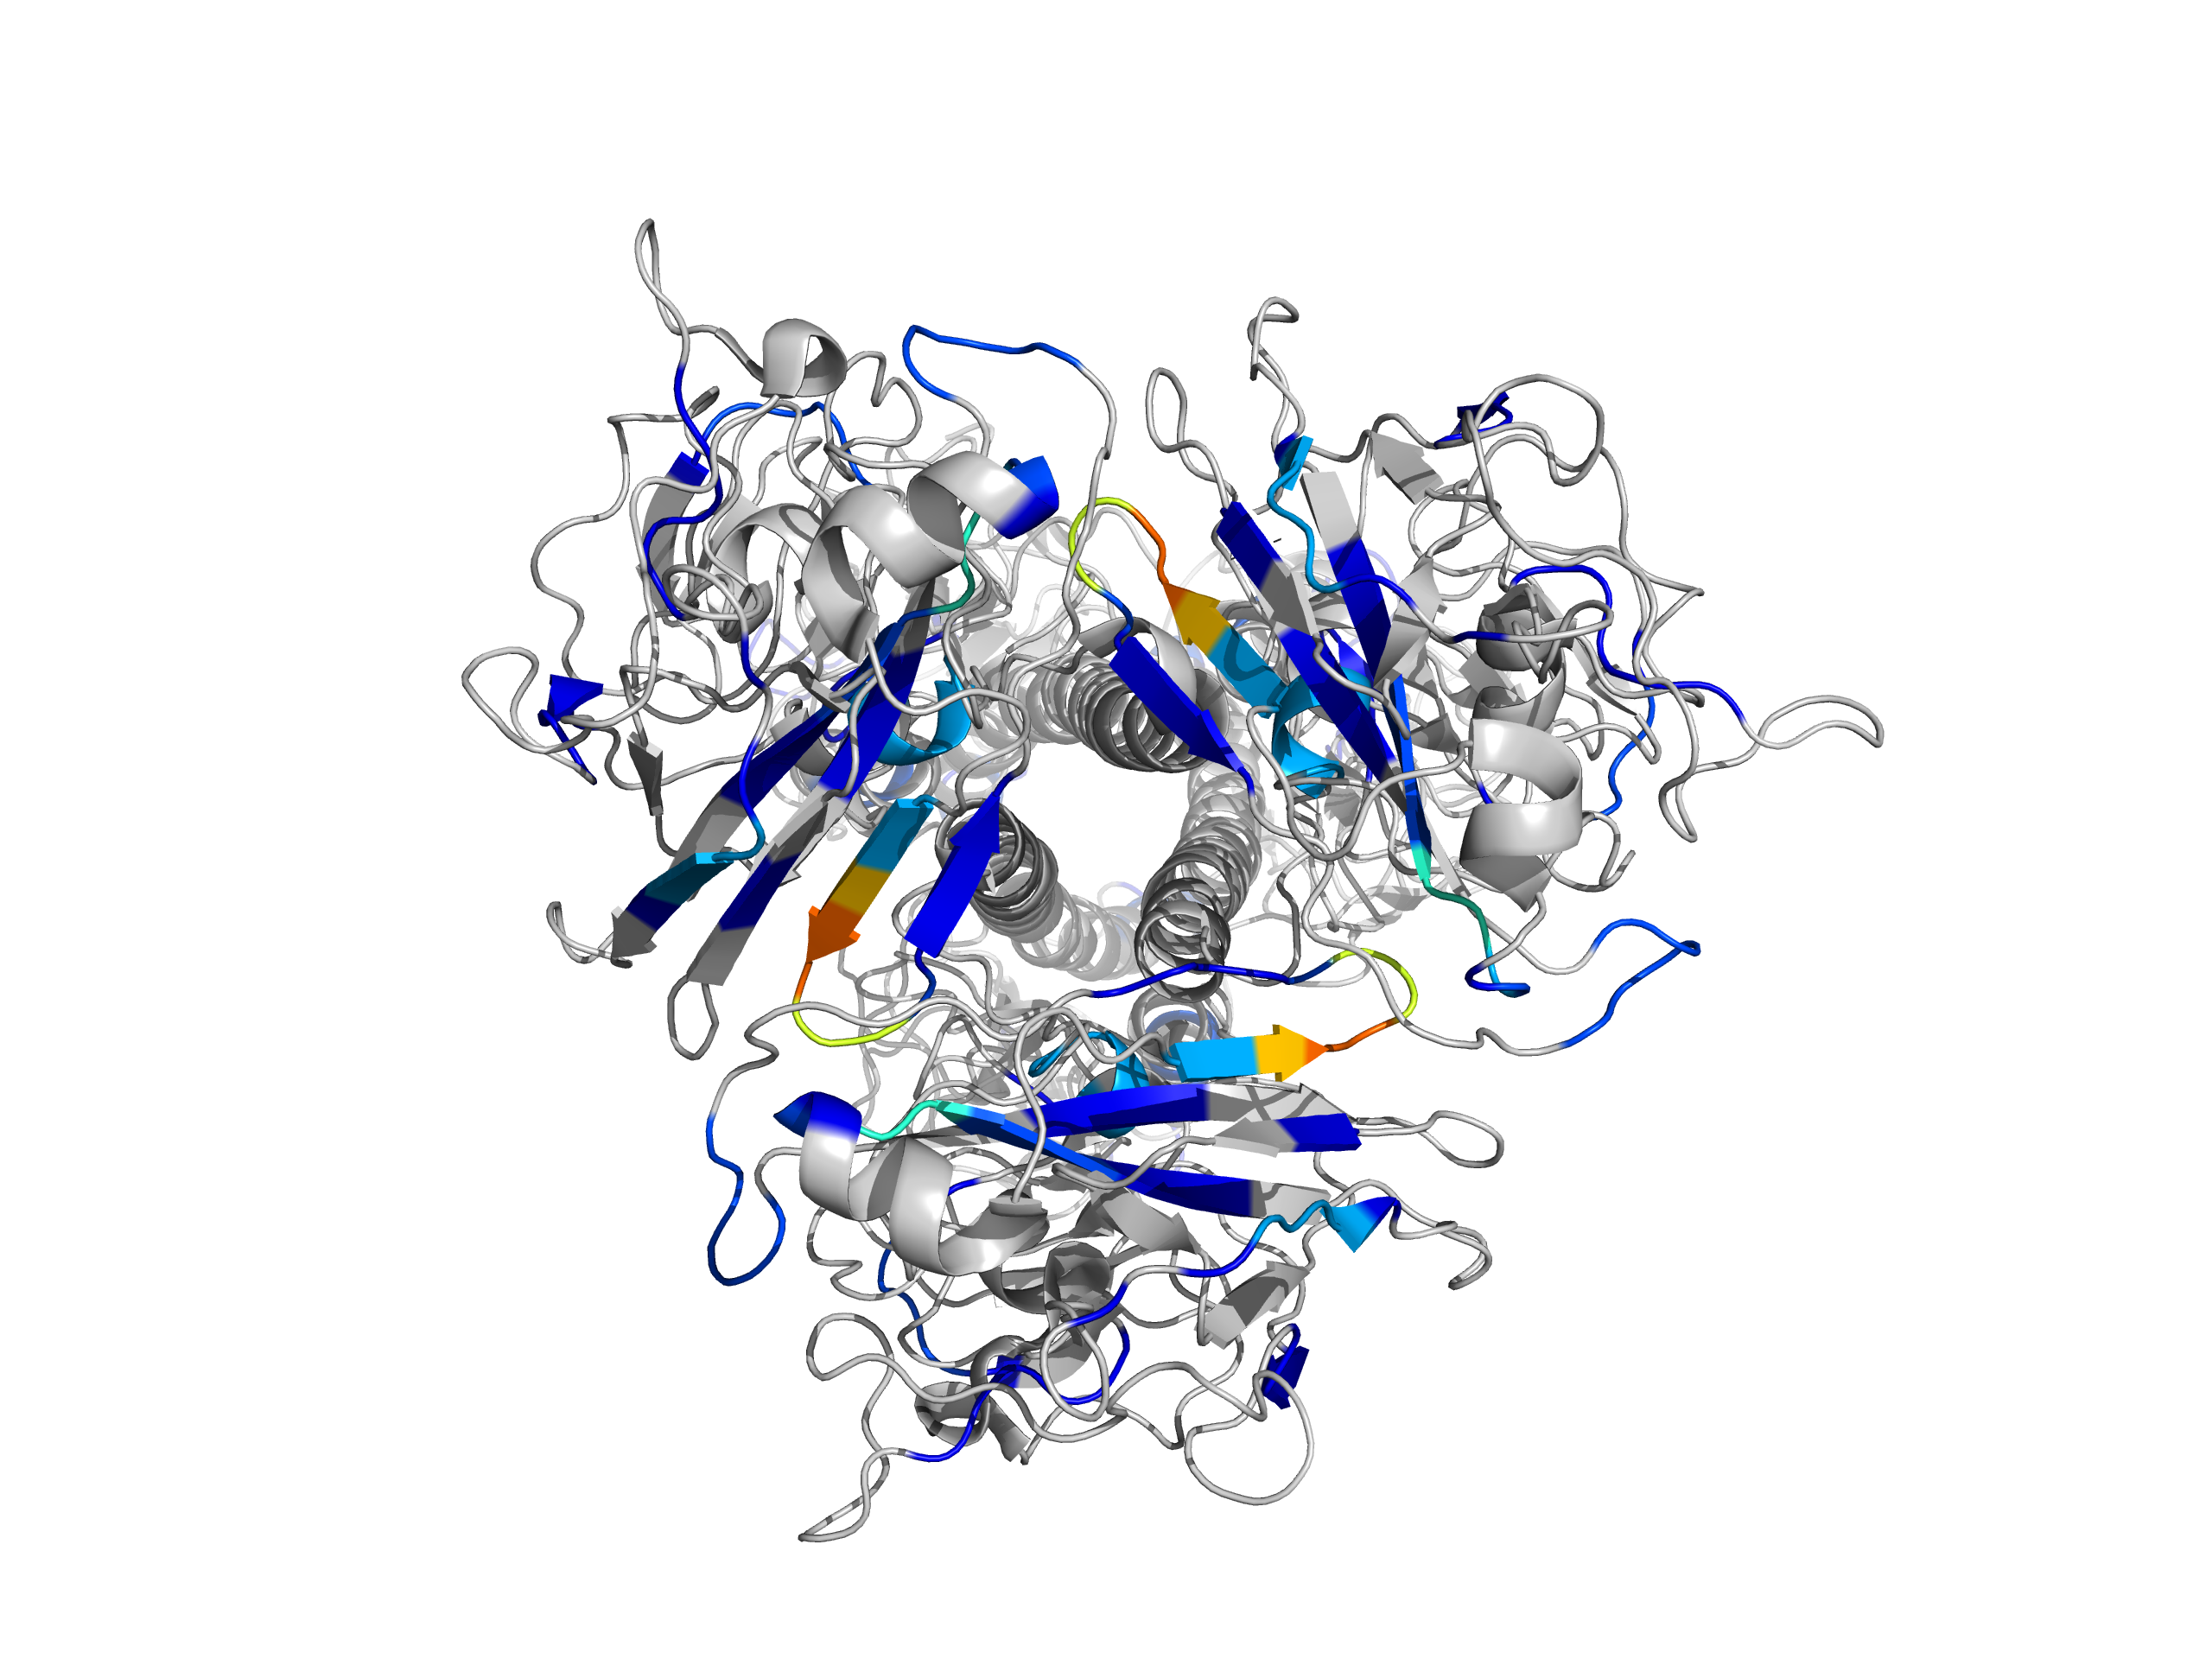
\includegraphics[width=2.75in]{/home/ishanu/ZED/Research/publications/pub_pan_one_/Figures/plotdata/seqanal/ntb/jetrndfile1.png}};
 \node[anchor=north west] (T111) at ([yshift=-0.15in,xshift=0.05in]T11.south west) {
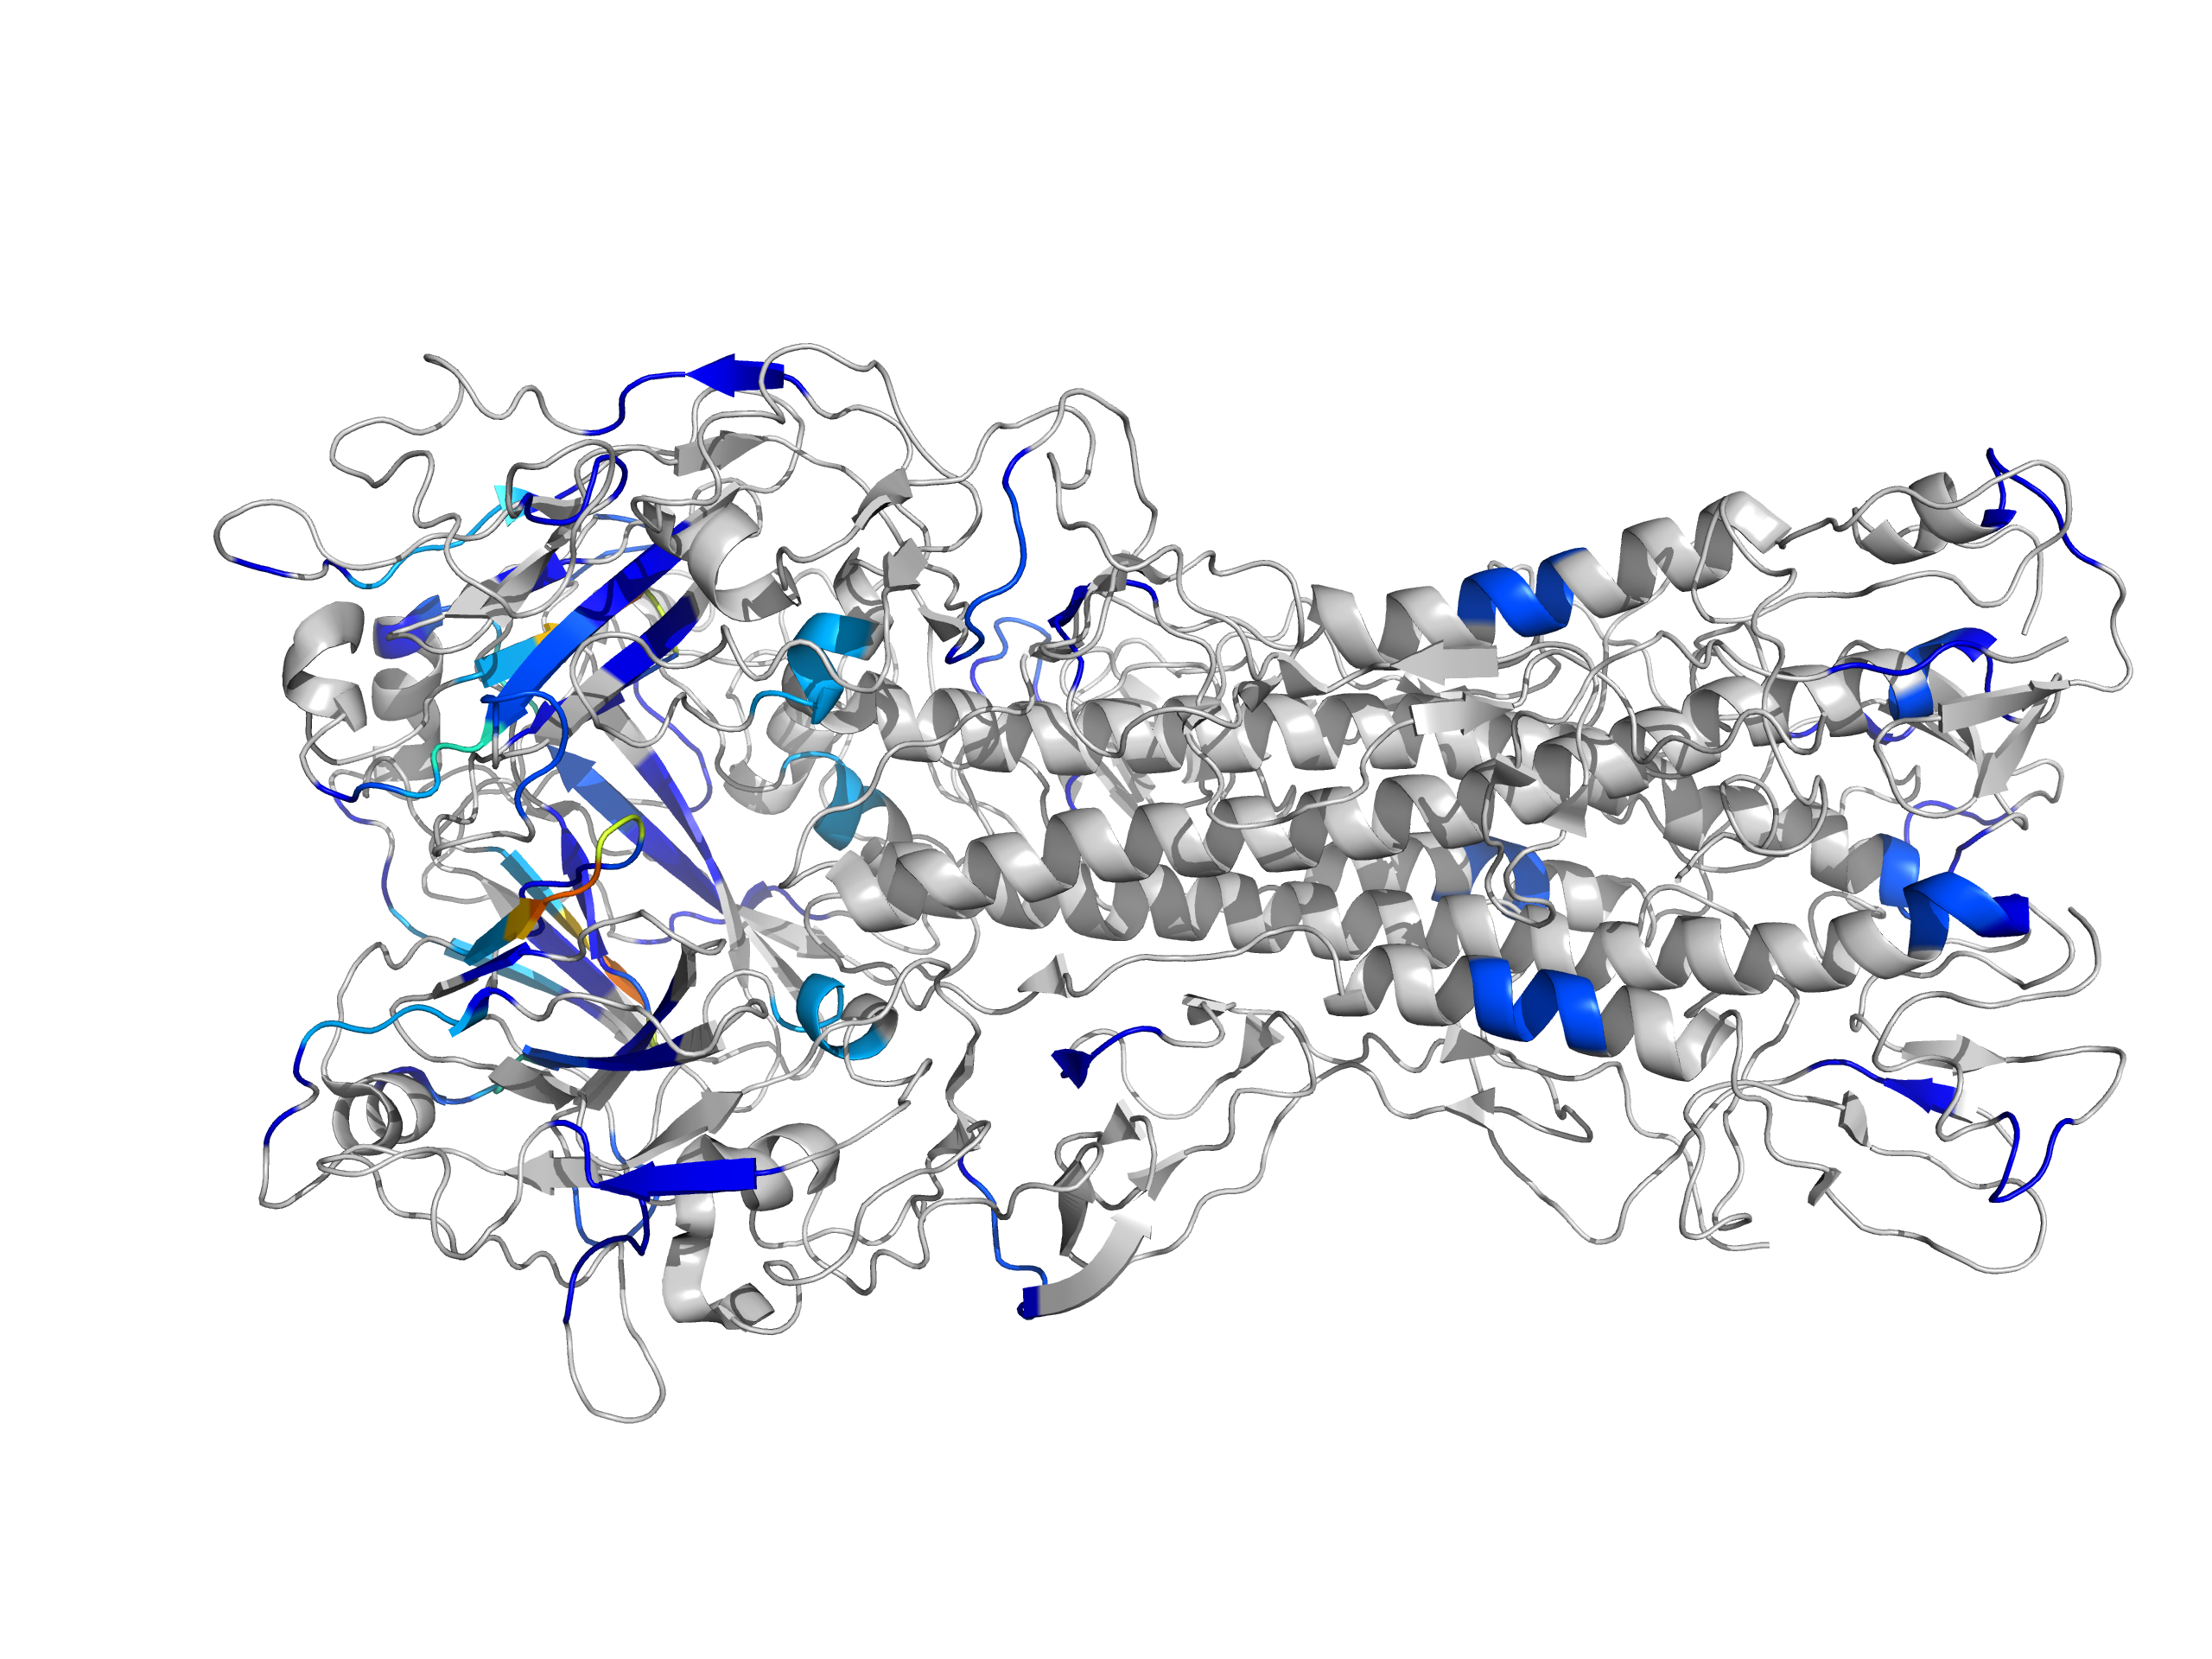
\includegraphics[width=3.5in,angle=-90]{/home/ishanu/ZED/Research/publications/pub_pan_one_/Figures/plotdata/seqanal/ntb/jetrndfile2.png}};
 \node[anchor=north west] (T112) at ([yshift=0.2in,xshift=.86in]T11.south west) {
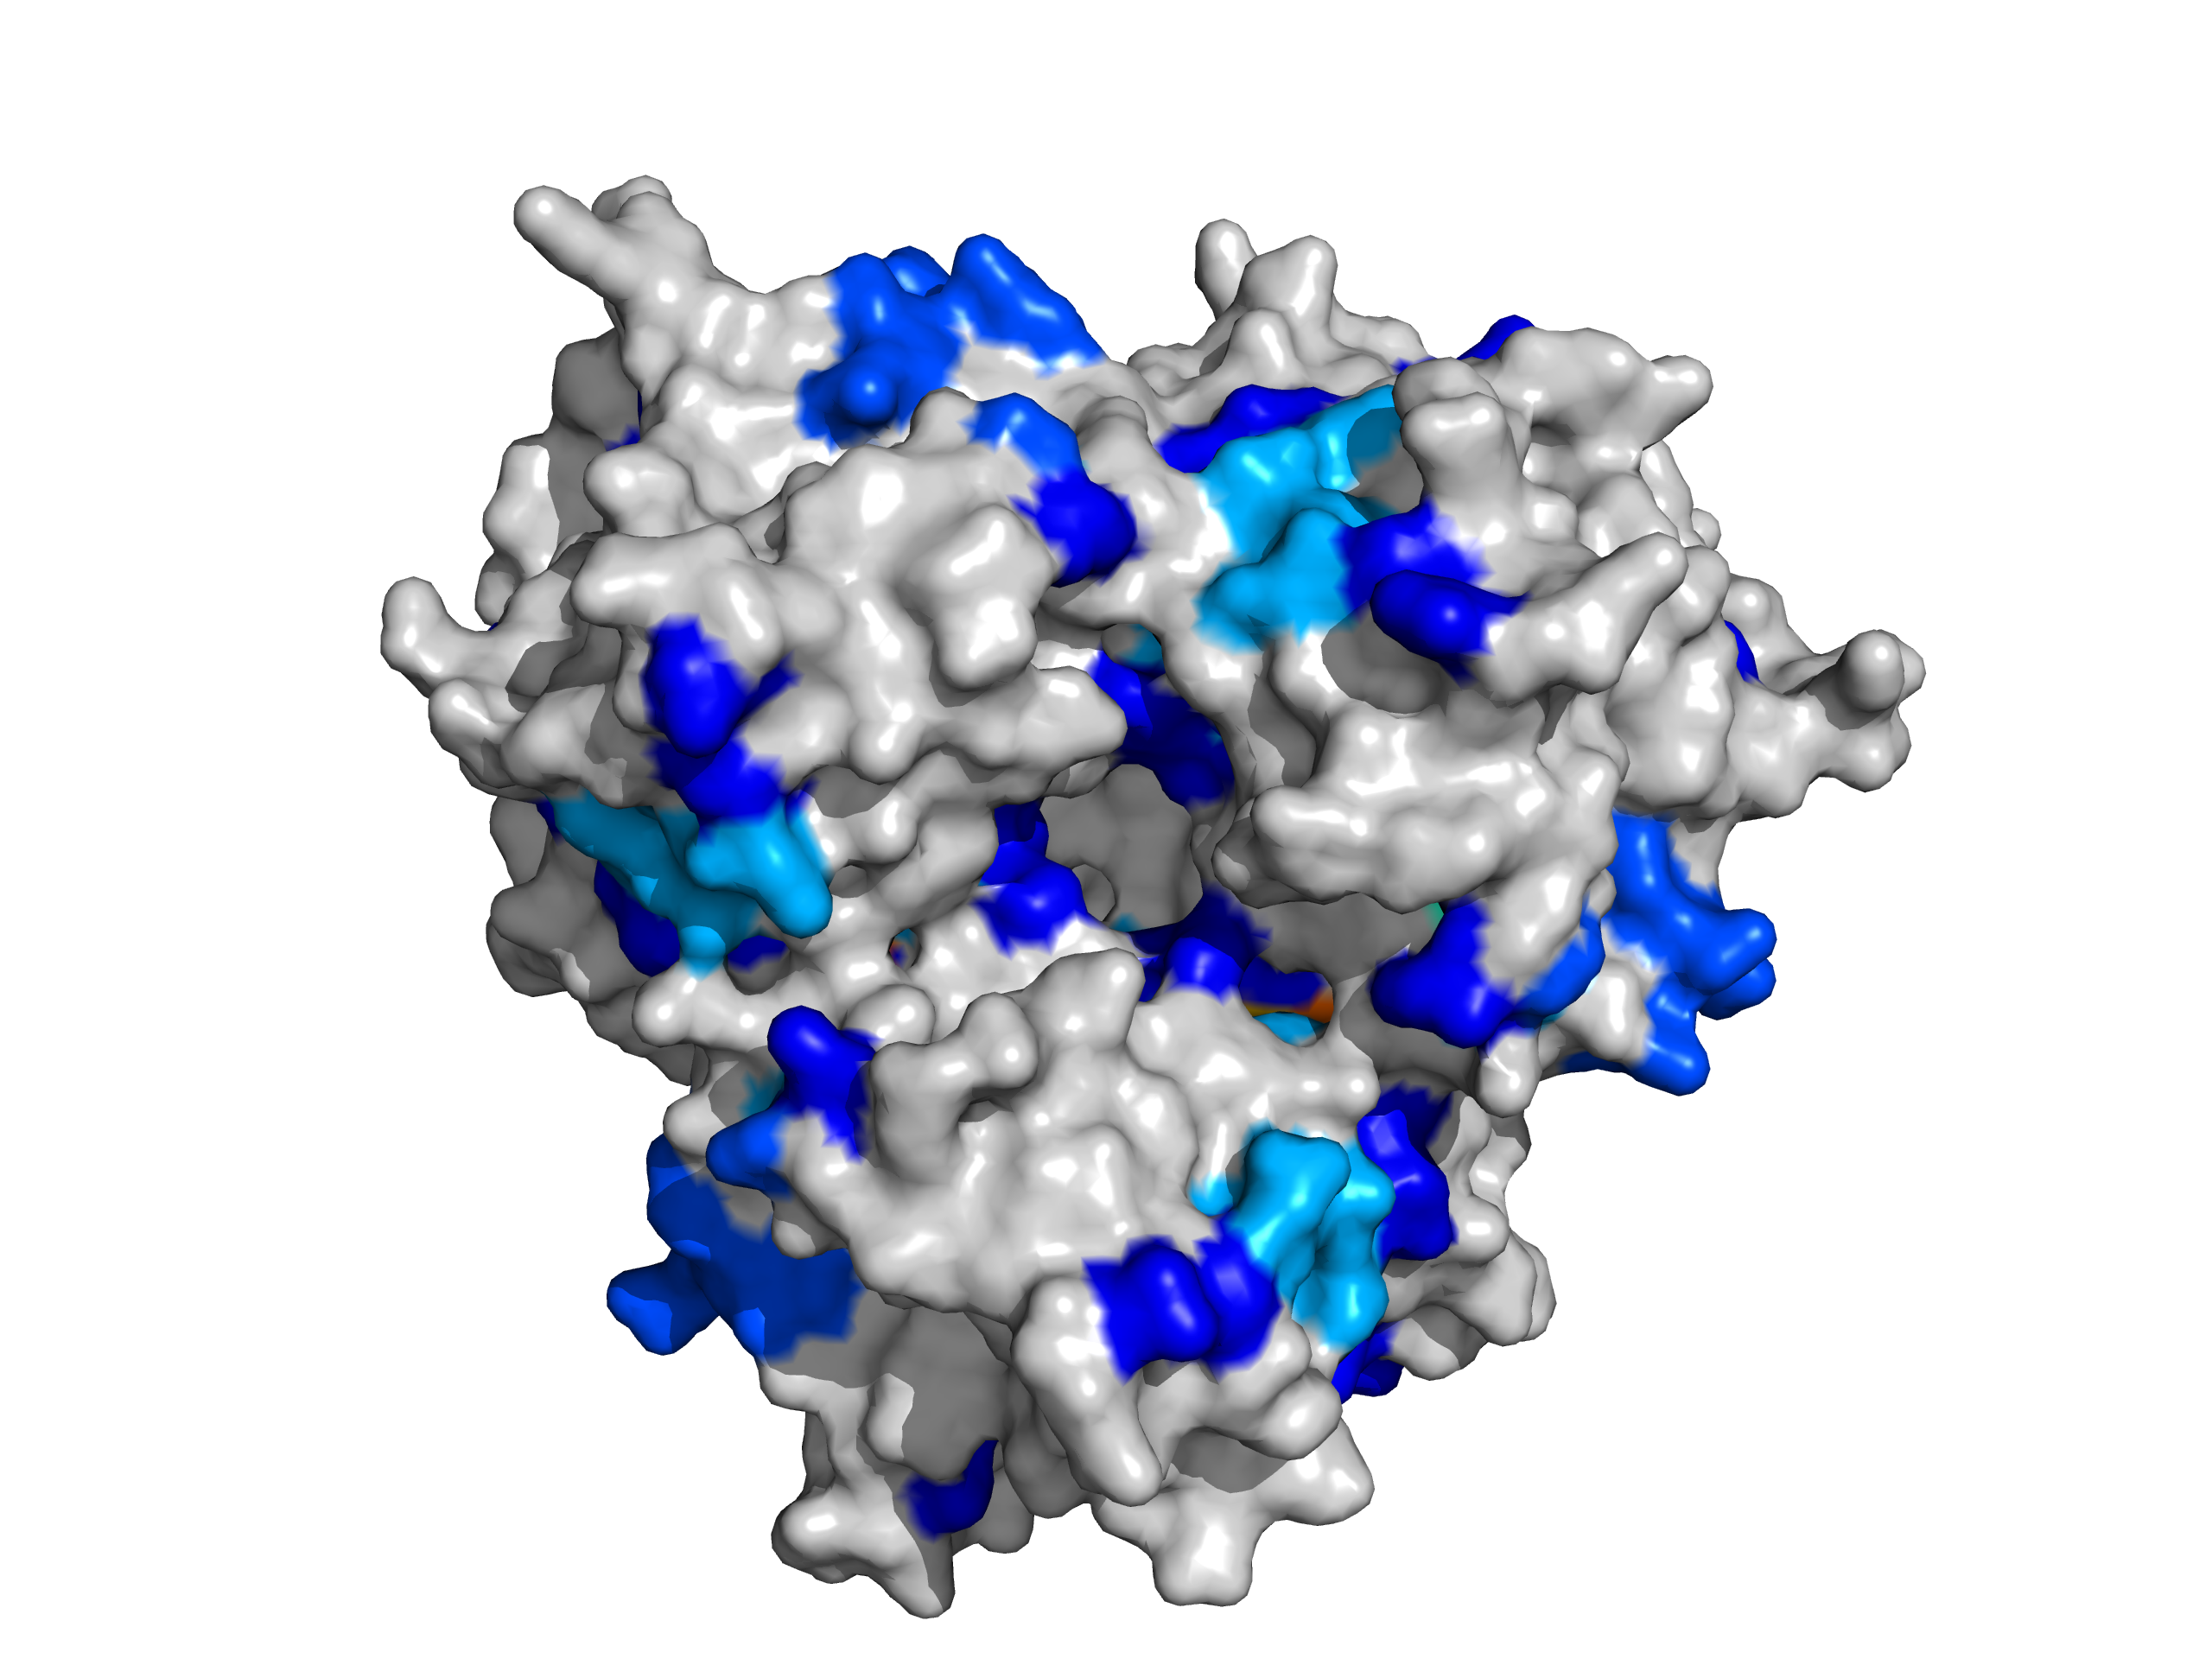
\includegraphics[width=1in]{/home/ishanu/ZED/Research/publications/pub_pan_one_/Figures/plotdata/seqanal/ntb/jetrndfile4.png}};
   

 \node[anchor=north west] (L2) at ([xshift=.6in,yshift=-0.05in]$(T1.north west)!(T11.west)!(T1.north east)$) {{\large \normalfont g.}};
 \node[anchor=north west] (L3) at ([xshift=.6in,yshift=-.1in]$(T11.north west)!(T112.north)!(T11.south west)$) {{\large \normalfont h.}};
 \node[anchor=north west] (L4) at ([xshift=.6in,yshift=-.45in]$(T11.north west)!(T111.north)!(T11.south west)$) {{\large \normalfont i.}};

\draw [thin, dashed] (T11.center) -- (T111.center);
\draw [-{latex},thin,Red1] ([xshift=-.8in,yshift=-.5in]T11.center) -- ([xshift=-.38in,yshift=-.17in]T11.center) node [pos=0.1,xshift=-.15in,yshift=-.02in,font=\bf\sffamily\fontsize{6}{6}\selectfont,text=black] {200} ;
\draw [-{latex},thin,Red1] ([xshift=-.8in,yshift=-.5in]T11.center) -- ([xshift=-0.12in,yshift=-2.1in]T11.center);
\draw [-{latex},thin,Red1] ([xshift=.6in,yshift=-.65in]T11.center) -- ([xshift=.3in,yshift=-.29in]T11.center) node [pos=-0.15,font=\bf\sffamily\fontsize{6}{6}\selectfont,text=black,fill=white] {200};
\draw [-{latex},thin,Red1] ([xshift=.1in,yshift=.7in]T11.center) -- ([xshift=.1in,yshift=.34in]T11.center) node [pos=-0.15,font=\bf\sffamily\fontsize{6}{6}\selectfont,text=black,fill=white] {200};

\draw [-{latex},thin,Red1] ([xshift=.73in,yshift=-.45in]T11.center) -- ([xshift=.7in,yshift=-.2in]T11.center) node [pos=-0.15,font=\bf\sffamily\fontsize{6}{6}\selectfont,text=black,fill=white] {220};

\draw [-{latex},thin,Red1] ([xshift=.73in,yshift=-.45in]T11.center) -- ([xshift=.7in,yshift=-.2in]T11.center) node [pos=-0.15,font=\bf\sffamily\fontsize{6}{6}\selectfont,text=black,fill=white] {220};

\draw [-{latex},thin,Red1] ([xshift=.53in,yshift=-.35in]T11.center) -- ([xshift=.42in,yshift=-0.1in]T11.center) node [pos=-0.15,font=\bf\sffamily\fontsize{6}{6}\selectfont,text=black] {180};

\draw [-{latex},thin,Red1] ([xshift=.53in,yshift=-.35in]T111.center) -- ([xshift=.42in,yshift=-0.6in]T111.center) node [pos=-0.15,xshift=.05in,font=\bf\sffamily\fontsize{6}{6}\selectfont,text=black] {49(HA2)};

\draw [-{latex},thin,Red1] ([xshift=-.8in,yshift=-.15in]T111.center) -- ([xshift=-.35in,yshift=0.4in]T111.center) node [pos=-0.15,xshift=.05in,font=\bf\sffamily\fontsize{6}{6}\selectfont,text=black] {100};

\draw [-{latex},thin,Red1] ([xshift=-1in,yshift=.2in]T111.center) -- ([xshift=-.6in,yshift=0.65in]T111.center) node [pos=-0.15,xshift=.05in,font=\bf\sffamily\fontsize{6}{6}\selectfont,text=black] {115};

\draw [-{latex},thin,Red1] ([xshift=-.8in,yshift=-1.1in]T111.center) -- ([xshift=-0.1in,yshift=-1.32in]T111.center) node [pos=-0.15,xshift=.05in,yshift=.01in,font=\bf\sffamily\fontsize{6}{6}\selectfont,text=black] {124 (HA2)};

\node[fill=white,  opacity=.65] (CC) at ([xshift=.1in,yshift=.02in]T112.east) {\begin{tikzpicture}
\begin{axis}[font=\bf\sffamily\fontsize{6}{6}\selectfont,
  hide axis,major tick length=0pt,
  xtick=\empty,
    scale only axis,
    height=0pt,
    width=0pt,
    colormap/jet,
    colorbar,
    point meta min=0.01,
    point meta max=0.11,
    colorbar style={title={frequency},title style={yshift=-.05in},font=\bf\sffamily\fontsize{6}{6}\selectfont,draw=none,axis line style={white}, y tick label style={
        /pgf/number format/.cd,
            fixed,
            fixed zerofill,
            precision=2,
        /tikz/.cd
    },  height=.5in,width=.1in,
        ytick={0.01,0.06,0.11}
    }]
    \addplot [draw=none] coordinates {(0,0)};
\end{axis}
\end{tikzpicture}};
  % \node[anchor=north west,label={[]90:{\large b.} 2018-2019 (Northern Hemisphere)}] (T2) at ([xshift=.1in]T1.south west) {
  %   \begin{tikzpicture}[font=\bf\sffamily\fontsize{7}{7}\selectfont]
  %     \node[] (A) at (0,0) {
  %       \mnp{2.65in}{\begin{texshade}{\SEQB}
  %           \shadingmode[chemical]{functional}
  %           \hideallmatchpositions
  %           \rulersteps{1}
  %           \setfont{residues}{sf}{up}{bf}{tiny} 
  %           \setfont{numbering}{sf}{up}{bf}{tiny} 
  %           \setfont{names}{tt}{up}{bf}{small}
  %           \setfont{legend}{tt}{up}{bf}{scriptsize}
  %           \threshold[80]{50}
  %           \setends{1}{1..\LENA}
  %           \showruler{1}{top}
  %           \hideconsensus
  %           \shadeallresidues
  %           \showlegend
  %         \end{texshade}
  %         % 
  %         \begin{texshade}{\SEQB}
  %           %\shadingmode[standard area]{functional}
  %           \shadingmode[hydropathy]{functional}
  %           \hideallmatchpositions
  %           \rulersteps{1}
  %           \setfont{residues}{sf}{up}{bf}{tiny} 
  %           \setfont{numbering}{sf}{up}{bf}{tiny} 
  %           \setfont{names}{tt}{up}{bf}{small}
  %           \setfont{legend}{tt}{up}{bf}{scriptsize}
  %           \threshold[80]{50}
  %           \setends{1}{1..\LENA}
  %           \showruler{1}{top}
  %           \hideconsensus
  %           \shadeallresidues
  %           \showlegend
  %         \end{texshade}
  %         % 
  %         \begin{texshade}{\SEQB}
  %           \shadingmode[accessible area]{functional}
  %           \hideallmatchpositions
  %           \rulersteps{1}
  %           \setfont{residues}{sf}{up}{bf}{tiny}
  %           \setfont{numbering}{sf}{up}{bf}{tiny} 
  %           \setfont{names}{tt}{up}{bf}{small}
  %           \setfont{legend}{tt}{up}{bf}{scriptsize}
  %           \threshold[80]{50}
  %           \setends{1}{1..\LENA}
  %           \showruler{1}{top}
  %           \hideconsensus
  %           \shadeallresidues
  %           \showlegend
  %         \end{texshade}
  %         % 
  %       }};
  %   \end{tikzpicture}};

 %  \node[anchor=north west,label={[]90:{\large c.} 2016-2017 (Southern Hemisphere)}] (T2) at ([xshift=0in]T1.south west) {
%     \begin{tikzpicture}[font=\bf\sffamily\fontsize{7}{7}\selectfont]
%       \node[ ] (A) at (0,0) {
%         \mnp{3.5in}{\begin{texshade}{\SEQC}
%             %\shadingmode[chemical]{functional}
%             \shadingmode[accessible area]{functional}
%             \hideallmatchpositions
%             \rulersteps{1}
%             \setfont{residues}{sf}{up}{bf}{tiny} 
%             \setfont{numbering}{sf}{up}{bf}{tiny} 
%             \setfont{names}{tt}{up}{bf}{small}
%             \setfont{legend}{tt}{up}{bf}{scriptsize}
%             \threshold[80]{50}
%             \setends{1}{1..\LENA}
%             \showruler{1}{top}
%             \hideconsensus
%             \shadeallresidues
%             \showlegend
%           \end{texshade}}};
% \node[] (B) at (A.north east) {  \mnp{3.5in}{      
%           % 
%           \begin{texshade}{\SEQC}
%             %\shadingmode[standard area]{functional}
%             \shadingmode[hydropathy]{functional}
%             \hideallmatchpositions
%             \rulersteps{1}
%             \setfont{residues}{sf}{up}{bf}{tiny} 
%             \setfont{numbering}{sf}{up}{bf}{tiny} 
%             \setfont{names}{tt}{up}{bf}{small}
%             \setfont{legend}{tt}{up}{bf}{scriptsize}
%             \threshold[80]{50}
%             \setends{1}{1..\LENA}
%             \showruler{1}{top}
%             \hideconsensus
%             \shadeallresidues
%             \showlegend
%           \end{texshade}}};


      
%     \end{tikzpicture}};


  

  % \node[anchor=north west,label={[]90:{\large d.} 2016-2017 (Northern Hemisphere)}] (T4) at ([xshift=0in]T3.south west) {
  %   \begin{tikzpicture}[font=\bf\sffamily\fontsize{7}{7}\selectfont]
  %     \node[label={[yshift=-1in,xshift=.15in]170:\mnp{.4in}{\raggedright type \\ \vspace{35pt} sd. chn. area \\ \vspace{35pt} acc. sd. chn.}}] (A) at (0,0) {
  %       \mnp{3.2in}{\begin{texshade}{\SEQD}
  %           \shadingmode[chemical]{functional}
  %           \hideallmatchpositions
  %           \rulersteps{1}
  %           \setfont{residues}{sf}{up}{bf}{tiny} 
  %           \setfont{numbering}{sf}{up}{bf}{tiny} 
  %           \setfont{names}{tt}{up}{bf}{small}
  %           \setfont{legend}{tt}{up}{bf}{scriptsize}
  %           \threshold[80]{50}
  %           \setends{1}{1..\LENA}
  %           \showruler{1}{top}
  %           \hideconsensus
  %           \shadeallresidues
  %           % \showlegend
  %         \end{texshade}
  %         % 
  %         \begin{texshade}{\SEQD}
  %           %\shadingmode[standard area]{functional}
  %           \shadingmode[hydropathy]{functional}
  %           \hideallmatchpositions
  %           \rulersteps{1}
  %           \setfont{residues}{sf}{up}{bf}{tiny} 
  %           \setfont{numbering}{sf}{up}{bf}{tiny} 
  %           \setfont{names}{tt}{up}{bf}{small}
  %           \setfont{legend}{tt}{up}{bf}{scriptsize}
  %           \threshold[80]{50}
  %           \setends{1}{1..\LENA}
  %           \showruler{1}{top}
  %           \hideconsensus
  %           \shadeallresidues
  %           % \showlegend
  %         \end{texshade}
  %         % 
  %         \begin{texshade}{\SEQD}
  %           \shadingmode[accessible area]{functional}
  %           \hideallmatchpositions
  %           \rulersteps{1}
  %           \setfont{residues}{sf}{up}{bf}{tiny}
  %           \setfont{numbering}{sf}{up}{bf}{tiny} 
  %           \setfont{names}{tt}{up}{bf}{small}
  %           \setfont{legend}{tt}{up}{bf}{scriptsize}
  %           \threshold[80]{50}
  %           \setends{1}{1..\LENA}
  %           \showruler{1}{top}
  %           \hideconsensus
  %           \shadeallresidues
  %           % \showlegend
  %         \end{texshade}
  %         % 
  %       }};
  %   \end{tikzpicture}};



  % \node[anchor=north west,label={[]90:{\large e.} 2016-2017 (H3N2 Northern Hemisphere)}] (T5) at ([xshift=0in]T4.south west) {
  %   \begin{tikzpicture}[font=\bf\sffamily\fontsize{7}{7}\selectfont]
  %     \node[label={[yshift=-1in,xshift=.15in]170:\mnp{.4in}{\raggedright type \\ \vspace{35pt} sd. chn. area \\ \vspace{35pt} acc. sd. chn.}}] (A) at (0,0) {
  %       \mnp{3.2in}{\begin{texshade}{\SEQE}
  %           \shadingmode[chemical]{functional}
  %           \hideallmatchpositions
  %           \rulersteps{1}
  %           \setfont{residues}{sf}{up}{bf}{tiny} 
  %           \setfont{numbering}{sf}{up}{bf}{tiny} 
  %           \setfont{names}{tt}{up}{bf}{small}
  %           \setfont{legend}{tt}{up}{bf}{scriptsize}
  %           \threshold[80]{50}
  %           \setends{1}{1..\LENA}
  %           \showruler{1}{top}
  %           \hideconsensus
  %           \shadeallresidues
  %           % \showlegend
  %         \end{texshade}
  %         % 
  %         \begin{texshade}{\SEQE}
  %           %\shadingmode[standard area]{functional}
  %           \shadingmode[hydropathy]{functional}
  %           \hideallmatchpositions
  %           \rulersteps{1}
  %           \setfont{residues}{sf}{up}{bf}{tiny} 
  %           \setfont{numbering}{sf}{up}{bf}{tiny} 
  %           \setfont{names}{tt}{up}{bf}{small}
  %           \setfont{legend}{tt}{up}{bf}{scriptsize}
  %           \threshold[80]{50}
  %           \setends{1}{1..\LENA}
  %           \showruler{1}{top}
  %           \hideconsensus
  %           \shadeallresidues
  %           % \showlegend
  %         \end{texshade}
  %         % 
  %         \begin{texshade}{\SEQE}
  %           \shadingmode[accessible area]{functional}
  %           \hideallmatchpositions
  %           \rulersteps{1}
  %           \setfont{residues}{sf}{up}{bf}{tiny}
  %           \setfont{numbering}{sf}{up}{bf}{tiny} 
  %           \setfont{names}{tt}{up}{bf}{small}
  %           \setfont{legend}{tt}{up}{bf}{scriptsize}
  %           \threshold[80]{50}
  %           \setends{1}{1..\LENA}
  %           \showruler{1}{top}
  %           \hideconsensus
  %           \shadeallresidues
  %           % \showlegend
  %         \end{texshade}
  %         % 
  %       }};
  %   \end{tikzpicture}};


  
\end{tikzpicture}  
  \vspace{0pt}   
  
  \else
  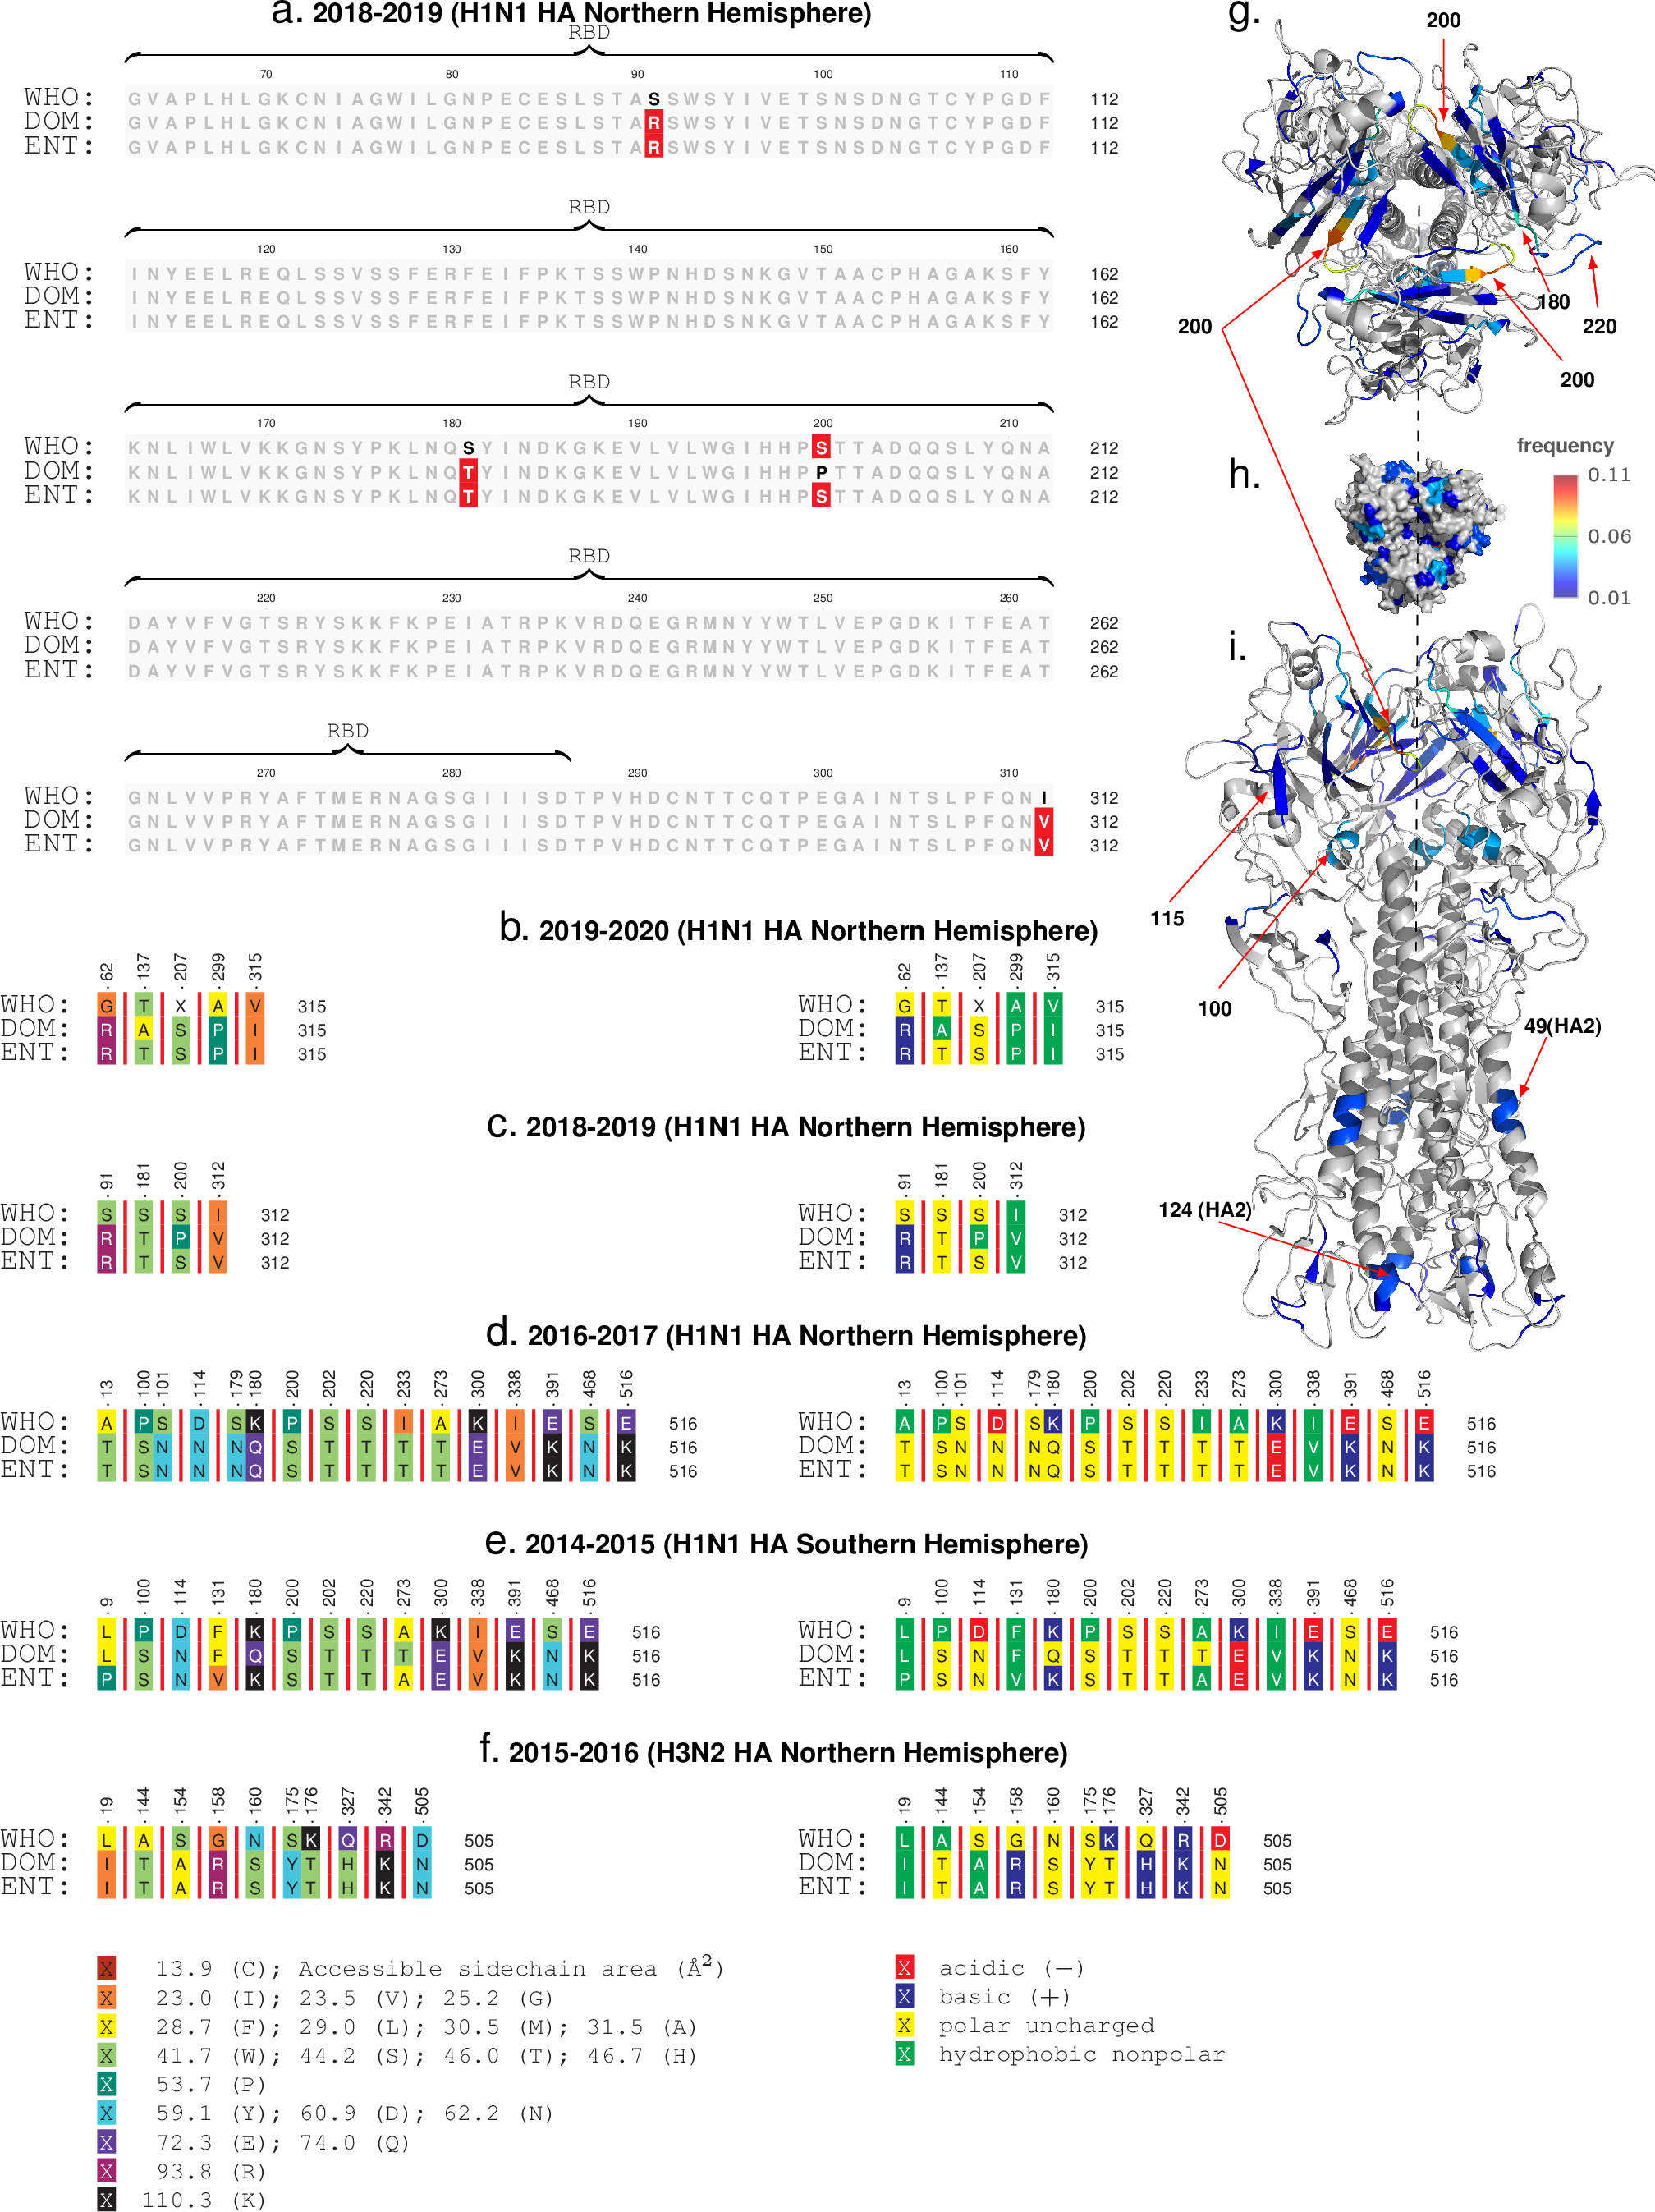
\includegraphics[width=0.87\textwidth]{Figures/External/sequence.pdf}  \vspace{-5pt}   

  \fi
  
\vspace{0pt}

\captionN{\textbf{Sequence comparisons.} Comparing the \enet  (ENT) and the WHO recommendation (WHO), and the observed dominant strain (DOM), we note that the correct \enet  predictions tend to be within the RBD, both for H1N1 and H3N2 for HA (panel a shows one example). Additionally, by comparing the type, side chain area, and the accessible side chain area, we note that DOM and ENT are often close in important chemical properties, while WHO deviations are  not (panel b-f). Panels g-i show the localization of the deviations in the molecular structure of HA, where we note that the changes are most frequent in the HA1 sub-unit (the globular head), and around residues and structures that have been commonly implicated in receptor binding interactions $e.g$ the $\approx 200$ loop, the $\approx 220$ loop and the $\approx 180$-helix~\cite{tzarum2015structure,lazniewski2018structural,garcia2015dynamic}.}\label{figseq}
\end{figure*}
\else
\refstepcounter{figure}\label{figseq}
\fi
%#############################################
%#############################################
%#############################################
\ifFIGS

\begin{table}[!ht]\centering
\captionN{Influenza A Strains Evaluated by IRAT and Corresponding \enet Computed Risk Scores}\label{irattab}

\sffamily\fontsize{7}{8}\selectfont

\begin{tabular}{L{1.25in}|L{.35in}|L{.3in}|L{.3in}|L{.3in}|L{.35in}|L{.35in}|L{.35in}|L{.35in}|L{.32in}|L{.3in}|L{.3in}}\hline
Influenza Virus & Subype & IRAT Date &IRAT Emergence Score &IRAT Impact Score &HA Sample &NA Sample &HA \erisk & NA \erisk &Geom. Mean&\qnet Emergence Score&\qnet Impact Score \\\hline
 A/swine/Shandong/1207/2016 &H1N1& Jul  2020 &7.5&6.9&1000&1000&-0.0941&-0.0205&0.0440&6.0&6.2\\\hline
 A/Ohio/13/2017 &H3N2& Jul  2019 &6.6&5.8&1000&1000&-0.0184&-0.0306&0.0238&6.3&6.2\\\hline
 A/Hong  Kong/125/2017 &H7N9& May  2017 &6.5&7.5&437&437&-0.0296&-0.0058&0.0131&6.6&6.5\\\hline
 A/Shanghai/02/2013 &H7N9& Apr  2016 &6.4&7.2&178&178&-0.0055&-0.0036&0.0044&6.7&6.6\\\hline
 A/Anhui-Lujiang/39/2018 &H9N2& Jul  2019 &6.2&5.9&31&30&-0.0290&-0.1681&0.0698&5.2&5.0\\\hline
 A/Indiana/08/2011 &H3N2& Dec  2012 &6.0&4.5&1000&1000&-0.0523&-0.0091&0.0218&6.4&6.5\\\hline
 A/California/62/2018 &H1N2& Jul  2019 &5.8&5.7&55&55&-0.1089&-0.0610&0.0815&5.4&5.5\\\hline
 A/Bangladesh/0994/2011$^{\star\star\star}$ &H9N2& Feb  2014 &5.6&5.4&&&-0.2078&-0.1823&0.1947&4.3&4.9\\\hline
 A/Sichuan/06681/2021 &H5N6& Oct  2021 &5.3&6.3&45&45&-0.3616&-0.0518&0.1369&5.2&6.4\\\hline
 A/Vietnam/1203/2004 &H5N1& Nov  2011 &5.2&6.6&258&246&-0.1673&-0.0111&0.0430&6.2&6.7\\\hline
 A/Yunnan/14564/2015$^{\star\star}$ &H5N6& Apr  2016 &5.0&6.6&344&331&-0.3482&-0.2987&0.3225&4.9&6.5\\\hline
 A/Astrakhan/3212/2020$^{\star\star}$ &H5N8& Mar  2021 &4.6&5.2&381&365&-0.1603&-0.3472&0.2359&3.9&4.4\\\hline
 A/Netherlands/219/2003 &H7N7& Jun  2012 &4.6&5.8&46&46&-0.2757&-0.3521&0.3115&4.6&5.8\\\hline
 A/American  wigeon/South  Carolina/AH0195145/2021 &H5N1& Mar  2022 &4.4&5.1&335&323&-0.1722&-0.5114&0.2967&4.0&4.7\\\hline
 A/Jiangxi-Donghu/346/2013$^{\star\star\star}$ &H10N8& Feb  2014 &4.3&6.0&&&-0.2088&-0.2101&0.2094&4.3&4.8\\\hline
 A/gyrfalcon/Washington/ 41088/2014$^{\star\star}$ &H5N8& Mar  2015 &4.2&4.6&341&328&-0.1532&-0.3424&0.2290&3.9&4.3\\\hline
 A/Northern  pintail/ Washington/40964/2014$^{\star\star}$ &H5N2& Mar  2015 &3.8&4.1&341&328&-0.1529&-0.3799&0.2410&3.9&4.3\\\hline
 A/canine/Illinois/12191/2015 &H3N2& Jun  2016 &3.7&3.7&1000&1000&-0.0607&-0.1509&0.0957&4.9&4.8\\\hline
 A/American  green-winged  teal /Washington/1957050/2014 &H5N1& Mar 2015 &3.6&4.1&326&314&-0.1911&-0.4482&0.2927&4.1&4.9\\\hline
 A/turkey/Indiana/1573-2/2016$^{\star\star}$ &H7N8& Jul  2017 &3.4&3.9&495&494&-0.1130&-0.7738&0.2957&3.4&3.9\\\hline
 A/chicken/Tennessee/17-007431-3/2017 &H7N9& Oct  2017 &3.1&3.5&496&495&-0.1027&-0.2569&0.1624&4.1&4.2\\\hline
 A/chicken/Tennessee/17-007147-2/2017 &H7N9& Oct  2017 &2.8&3.5&496&495&-0.2095&-0.2541&0.2307&4.2&4.8\\\hline
% A/duck/New  York/1996 $^\star$&H1N1& Nov  2011 &2.3&2.4&1000&1000&-1&-1&-1&-1&-1\\\hline
 \end{tabular}
\flushleft

 \fontsize{8}{8}\selectfont
 $^{\star\star}$  \enet constructed using all human strains that match the HA sub-type, $e.g.$, H5Nx for H5N6.\\
 $^{\star\star\star}$ distance estaimated averaging over those obtained by considering all \enet{s} from other subtypes.
\end{table}
\else
\refstepcounter{table}\label{irattab}
\fi
% #############################################

%#############################################



\ifFIGS

\begin{table}[!ht]\centering
\captionN{Count of identified strains above estimated emergence risk threshold}\label{riskytab}

\sffamily\fontsize{7}{8}\selectfont

\begin{tabular}{L{.75in}|L{.25in}|L{.60in}|L{.6in}|L{.6in}|L{.6in}}\hline
subtype | risk&6.0&6.2&6.3&6.4&6.5\\\hline
H1N1&62&57&53&5&4\\
H3N2&11&11&11&4&1\\
H7N9&1&1&1&1&1\\
H9N2&1&1&0&0&0\\
\hline\end{tabular}

\end{table}
\else
\refstepcounter{table}\label{riskytab}
\fi
% #############################################
%#############################################
\ifFIGS

\begin{table}[!ht]\centering
\captionN{Influenza A Strains Evaluated by IRAT and Corresponding \enet Computed Risk Scores}\label{highrisktab}

\bf\sffamily\fontsize{7}{7}\selectfont

\begin{tabular}{L{1.95in}|L{.25in}|L{.60in}|L{.6in}|C{1in}|C{1in}}\hline
strain&subtype& HA  accession & NA  accession & predicted  IRAT  impact & predicted  IRAT  emergence \\
\rowcolor{Red3!20}A/swine/Shandong/1207/2016&H1N1&EPI1751427&EPI1751500&6.9000&7.5000\\
\rowcolor{Red3!20}A/swine/Missouri/A02524711/2020&H1N1&EPI1818121&EPI1818122&6.7673&6.7822\\
\rowcolor{Blue1!30}A/swine/Indiana/A02524710/2020&H3N2&EPI1818137&EPI1818138&6.7205&6.7293\\
\rowcolor{Red3!20}A/swine/North\_Carolina/A02479173/2020&H1N1&EPI1780425&EPI1780426&6.7136&6.7215\\
\rowcolor{Green3!50}A/Camel/Inner\_Mongolia/XL/2020&H7N9&EPI2026200&EPI2026202&6.6990&6.7049\\
\rowcolor{Red3!20}A/swine/Tennessee/A02524414/2022&H1N1&EPI2149257&EPI2149258&6.6501&6.6494\\
\rowcolor{Blue1!30}A/Ohio/13/2017&H3N2&EPI1056653&EPI1056652&5.8000&6.6000\\
\rowcolor{Red3!20}A/swine/Minnesota/A02635976/2021&H1N1&EPI1912208&EPI1912209&6.5776&6.5670\\
\rowcolor{Blue1!30}A/swine/Chile/VN1401-5054/2020&H3N2&EPI1974975&EPI1974978&6.5318&6.5149\\
\rowcolor{Blue1!30}A/swine/Italy/56910/2020&H3N2&EPI2142217&EPI2142173&6.5292&6.5119\\
\rowcolor{Blue1!30}A/swine/Minnesota/A02245643/2020&H3N2&EPI1769178&EPI1769179&6.5067&6.4863\\
\rowcolor{Red3!20}A/swine/Iowa/A02479005/2020&H1N1&EPI1777621&EPI1777622&6.4872&6.4641\\
\rowcolor{Blue1!30}A/swine/Iowa/A02524878/2020&H3N2&EPI1907866&EPI1907867&6.4566&6.4291\\
\rowcolor{Red3!20}A/swine/Indiana/A02636638/2022&H1N1&EPI2153370&EPI2153371&6.4534&6.4255\\
\rowcolor{Blue1!30}A/swine/Iowa/A02524874/2020&H3N2&EPI1907838&EPI1907839&6.4392&6.4093\\
\rowcolor{Red3!20}A/swine/Minnesota/A02248037/2021&H1N1&EPI1912188&EPI1912189&6.4366&6.4063\\
\rowcolor{Red3!20}A/swine/Iowa/A02635917/2021&H1N1&EPI1911753&EPI1911754&6.4356&6.4052\\
\rowcolor{Red3!20}A/swine/Illinois/A02635936/2021&H1N1&EPI1911791&EPI1911792&6.4347&6.4042\\
\rowcolor{Red3!20}A/swine/Minnesota/A02711801/2022&H1N1&EPI2153420&EPI2153421&6.4334&6.4027\\
\rowcolor{Red3!20}A/swine/South\_Dakota/A02524453/2020&H1N1&EPI1765555&EPI1765556&6.4321&6.4012\\
\rowcolor{Blue1!30}A/swine/Illinois/A02479007/2020&H3N2&EPI1777629&EPI1777630&6.4315&6.4005\\
\rowcolor{Red3!20}A/swine/Minnesota/A02248061/2021&H1N1&EPI1912494&EPI1912495&6.4278&6.3963\\
\rowcolor{Red3!20}A/swine/Iowa/A02524875/2020&H1N1&EPI1907858&EPI1907859&6.4260&6.3943\\
\rowcolor{Blue1!30}A/swine/Spain/44579-1/2020&H3N2&EPI1930744&EPI1930748&6.4255&6.3937\\
\rowcolor{Red3!20}A/swine/Iowa/A02636439/2022&H1N1&EPI2147475&EPI2147476&6.4250&6.3931\\
\rowcolor{Red3!20}A/swine/Minnesota/A02248060/2021&H1N1&EPI1912500&EPI1912501&6.4234&6.3913\\
\rowcolor{Red3!20}A/swine/Nebraska/A02636117/2021&H1N1&EPI1932937&EPI1932938&6.4226&6.3903\\
\rowcolor{Red3!20}A/swine/Iowa/A02524513/2020&H1N1&EPI1832647&EPI1832648&6.4223&6.3901\\
\rowcolor{Red3!20}A/swine/Iowa/A02479383/2020&H1N1&EPI1771027&EPI1771028&6.4222&6.3899\\
\rowcolor{Red3!20}A/swine/Nebraska/A02479212/2020&H1N1&EPI1775884&EPI1775885&6.4222&6.3899\\
\rowcolor{Red3!20}A/swine/Minnesota/A02479051/2020&H1N1&EPI1778572&EPI1778573&6.4222&6.3899\\
\rowcolor{Red3!20}A/swine/Minnesota/A02245424/2020&H1N1&EPI1780207&EPI1780208&6.4222&6.3899\\
\rowcolor{Red3!20}A/swine/Iowa/A02525345/2021&H1N1&EPI1910807&EPI1910808&6.4222&6.3899\\
\rowcolor{Red3!20}A/swine/Iowa/A02524646/2020&H1N1&EPI1817164&EPI1817165&6.4222&6.3899\\
\rowcolor{Red3!20}A/swine/Iowa/A02524724/2020&H1N1&EPI1818387&EPI1818388&6.4222&6.3899\\
\rowcolor{Red3!20}A/swine/Iowa/A02525313/2021&H1N1&EPI1910761&EPI1910762&6.4222&6.3899\\
\rowcolor{Red3!20}A/swine/Missouri/A02525065/2021&H1N1&EPI1908581&EPI1908582&6.4222&6.3899\\
\rowcolor{Red3!20}A/swine/Missouri/A02524951/2020&H1N1&EPI1908429&EPI1908430&6.4222&6.3899\\
\rowcolor{Red3!20}A/swine/Iowa/A02524994/2020&H1N1&EPI1908427&EPI1908428&6.4222&6.3899\\
\rowcolor{Red3!20}A/swine/Nebraska/A02524935/2020&H1N1&EPI1908118&EPI1908119&6.4222&6.3899\\
\rowcolor{Red3!20}A/swine/Iowa/A02524892/2020&H1N1&EPI1907881&EPI1907882&6.4222&6.3899\\
\rowcolor{Red3!20}A/swine/Nebraska/A02479337/2020&H1N1&EPI1769116&EPI1769117&6.4222&6.3899\\
\rowcolor{Red3!20}A/swine/Nebraska/A02479186/2020&H1N1&EPI1774141&EPI1774142&6.4220&6.3897\\
\rowcolor{Blue1!30}A/swine/Minnesota/A02245699/2020&H3N2&EPI1833007&EPI1833008&6.4220&6.3897\\
\rowcolor{Red3!20}A/swine/Iowa/A02479156/2020&H1N1&EPI1780249&EPI1780250&6.4216&6.3892\\
\rowcolor{Red3!20}A/swine/Iowa/A02479229/2020&H1N1&EPI1775914&EPI1775915&6.4215&6.3891\\
\rowcolor{Red3!20}A/swine/Iowa/A02479303/2020&H1N1&EPI1768639&EPI1768640&6.4207&6.3882\\
\rowcolor{Red3!20}A/swine/Minnesota/A02710691/2021&H1N1&EPI2146090&EPI2146091&6.4200&6.3874\\
\rowcolor{Red3!20}A/swine/Iowa/A02635881/2021&H1N1&EPI1911668&EPI1911669&6.4198&6.3872\\
\rowcolor{Red3!20}A/swine/Iowa/A02525354/2021&H1N1&EPI1910789&EPI1910790&6.4198&6.3872\\
\rowcolor{Red3!20}A/swine/Iowa/A02635823/2021&H1N1&EPI1911263&EPI1911264&6.4176&6.3847\\
\rowcolor{Red3!20}A/swine/Iowa/A02524739/2020&H1N1&EPI1818383&EPI1818384&6.4173&6.3843\\
\rowcolor{Red3!20}A/swine/Iowa/A02479141/2020&H1N1&EPI1780241&EPI1780242&6.4161&6.3829\\
\rowcolor{Red3!20}A/swine/Iowa/A02635965/2021&H1N1&EPI1912220&EPI1912221&6.4136&6.3801\\
\rowcolor{Red3!20}A/swine/Iowa/A02245587/2020&H1N1&EPI1775817&EPI1775818&6.4119&6.3781\\
\rowcolor{Red3!20}A/swine/Iowa/A02750621/2022&H1N1&EPI2161576&EPI2161577&6.4116&6.3779\\
\rowcolor{Red3!20}A/swine/Iowa/A02636496/2022&H1N1&EPI2148086&EPI2148087&6.4105&6.3765\\
\rowcolor{Blue1!30}A/swine/South\_Dakota/A02524914/2020&H3N2&EPI1908070&EPI1908071&6.4101&6.3761\\
\rowcolor{Red3!20}A/swine/Iowa/A02525217/2021&H1N1&EPI1909087&EPI1909088&6.4090&6.3748\\
\rowcolor{Red3!20}A/swine/Iowa/A02636145/2021&H1N1&EPI1932055&EPI1932930&6.4090&6.3748\\
\rowcolor{Red3!20}A/swine/Iowa/A02636114/2021&H1N1&EPI1931853&EPI1931854&6.4090&6.3748\\
\rowcolor{Red3!20}A/swine/Iowa/A02635871/2021&H1N1&EPI1911656&EPI1911657&6.4089&6.3747\\
\rowcolor{Red3!20}A/swine/Iowa/A02479067/2020&H1N1&EPI1778734&EPI1778735&6.4083&6.3741\\
\rowcolor{Red3!20}A/swine/Minnesota/A02246459/2021&H1N1&EPI1912518&EPI1912519&6.4061&6.3716\\
\rowcolor{Blue1!30}A/swine/Minnesota/A02711797/2022&H3N2&EPI2153382&EPI2153383&6.4029&6.3679\\
\rowcolor{Red3!20}A/swine/Minnesota/A02525348/2021&H1N1&EPI1910795&EPI1910796&6.3996&6.3641\\
\rowcolor{Red3!20}A/swine/Iowa/A02479343/2020&H1N1&EPI1769114&EPI1769115&6.3985&6.3628\\
\rowcolor{Blue1!30}A/swine/Illinois/A02525253/2021&H3N2&EPI1910375&EPI1910376&6.3974&6.3615\\
\rowcolor{Blue1!30}A/swine/Colorado/A02710706/2022&H3N2&EPI2176699&EPI2176700&6.3629&6.3221\\
\rowcolor{Red3!20}A/swine/Kansas/A02245381/2020(H1N1)&H1N1&EPI1777723&EPI1777724&6.3447&6.3013\\
\rowcolor{Blue1!30}A/canine/Texas/21-011409-001/2021&H3N2&EPI1896555&EPI1896557&6.3440&6.3005\\
\rowcolor{Blue1!30}A/swine/Iowa/A02525161/2021&H3N2&EPI1909023&EPI1909024&6.3342&6.2893\\
\rowcolor{Red3!20}A/swine/Iowa/A02246996/2021&H1N1&EPI2146133&EPI2146134&6.3269&6.2809\\
\rowcolor{Blue1!30}A/Muscovy\_duck/Vietnam/QN6297/2020&H3N2&EPI1974815&EPI1974818&6.3239&6.2775\\
\rowcolor{DarkOrange!40}A/mink/China/chick\_embryo/2020&H9N2&EPI2161544&EPI2161548&6.3188&6.2716\\
\hline\end{tabular}

\end{table}
\else
\refstepcounter{table}\label{highrisktab}
\fi
% #############################################

\ifFIGS

\begin{figure}[!ht]
  \tikzexternalenable
  \tikzsetnextfilename{riskyseq}
  \centering
 %\tikzXtrue
 
  
  \iftikzX  
  \begin{tikzpicture}[font=\bf\sffamily\fontsize{8}{8}\selectfont]
  \def\SEQA{Figures/plotdata/seqanal/risky4.fasta}
  \def\LENA{550}
  \def\LENB{63}
  \def\LENC{286}
  \def\LENE{1}
  \def\LEND{550}
  \def\COLM{jet}
  \def\rndfileA{rndfile1.png}
  \def\rndfileB{rndfile2.png}
  \def\rndfileC{rndfile3.png}
  
  \newcommand{\panelX}[2] {
    \begin{tikzpicture}[font=\bf\sffamily\fontsize{7}{7}\selectfont]
      \node[ ] (A) at (0,0) {
        \mnp{3.2in}{\begin{texshade}{#1}
            %\shadingmode[chemical]{functional}
            \shadingmode[accessible area]{functional}
            \hideallmatchpositions
            \rulersteps{1}
            \setfont{residues}{sf}{up}{bf}{tiny} 
            \setfont{numbering}{sf}{up}{bf}{tiny} 
            \setfont{names}{tt}{up}{bf}{small}
            \setfont{legend}{tt}{up}{bf}{scriptsize}
            \threshold[80]{50}
            \setends{1}{1..\LENA}
            \showruler{1}{top}
            \hideconsensus
            \shadeallresidues
            #2
          \end{texshade}}};
\node[] (B) at (A.north east) {  \mnp{3.5in}{      
          % 
          \begin{texshade}{#1}
            %\shadingmode[standard area]{functional}
            \shadingmode[hydropathy]{functional}
            \hideallmatchpositions
            \rulersteps{1}
            \setfont{residues}{sf}{up}{bf}{tiny} 
            \setfont{numbering}{sf}{up}{bf}{tiny} 
            \setfont{names}{tt}{up}{bf}{small}
            \setfont{legend}{tt}{up}{bf}{scriptsize}
            \threshold[80]{50}
            \setends{1}{1..\LENA}
            \showruler{1}{top}
            \hideconsensus
            \shadeallresidues
            #2
          \end{texshade}}};
    \end{tikzpicture}
    }

  %\clip (-2.4in,-7.35in) rectangle (4.4in,2.60in);
  \node[] (T1) at (0,0){  
    % 
    \begin{tikzpicture}
      \node [%,label={[yshift=-.2in]90:{% \large \sffamily \normalfont a.} Top risky strains (2020-2022 April)  HA sequence comparison with Dominant Human Strains (H1N1, H3N2)
      % }
      ]
      (A) at (0,0.0) {
        \mnp{\textwidth}{
          \begin{texshade}{\SEQA}
           \residuesperline*{70}
           \shadingmode[allmatchspecial]{identical}
            \shadingcolors{grays}
            \conservedresidues{White}{Red}{upper}{bf}
            \allmatchresidues{gray!50}{lightgray!10}{upper}{bf}
            \nomatchresidues{black}{lightgray!50}{upper}{bf}
            \setfont{residues}{sf}{up}{bf}{tiny} 
            \setfont{numbering}{sf}{up}{bf}{tiny} 
            \setfont{names}{tt}{up}{bf}{small}
            \setfont{legend}{tt}{up}{bf}{scriptsize}
            \setfont{features}{tt}{up}{bf}{scriptsize}
            \feature{top}{1}{\LENB..\LENC}{brace[black]}{RBD}
            % \threshold[80]{50}
            \setends{1}{\LENE..\LEND}
            \showruler{1}{top}
            \hideconsensus
            % \defconsensus{.}{lower}{upper}
             \showlegend
          \end{texshade}
          % 
        }};
    \end{tikzpicture}};

 % \node[anchor=north west,label={[yshift=-.1in]90:{\large \large \sffamily \normalfont b.} 2019-2020 (H1N1 HA Northern Hemisphere)}] (T21) at ([xshift=-0.08in]T1.south west) {\panelX{\SEQAA}{}};

 % \node[anchor=north west,label={[xshift=-.05in,yshift=-.05in]90:{\large \large \sffamily \normalfont c.} 2018-2019 (H1N1 HA Northern Hemisphere)}] (T2) at ([xshift=-0.0in]T21.south west) {\panelX{\SEQB}{}};

 % \node[anchor=north west,label={[xshift=-.05in,yshift=-.05in]90:{\large \large \sffamily \normalfont d.} 2016-2017 (H1N1 HA Northern Hemisphere)}] (T3) at ([xshift=-0.0in]T2.south west) {\panelX{\SEQC}{}};

 % \node[anchor=north west,label={[xshift=-.05in,yshift=-.05in]90:{\large \large \sffamily \normalfont e.} 2014-2015 (H1N1 HA Southern Hemisphere)}] (T4) at ([xshift=-0.0in]T3.south west) {\panelX{\SEQD}{}};

 % \node[anchor=north west,label={[xshift=-.1in,yshift=-.05in]90:{\large \large \sffamily \normalfont f.} 2015-2016 (H3N2 HA Northern Hemisphere)}] (T5) at ([xshift=-0.0in]T4.south west) {\panelX{\SEQE}{\showlegend}};


%  \node[anchor=north west] (T11) at ([xshift=-.45in,yshift=0.15in]T1.north east) {
% 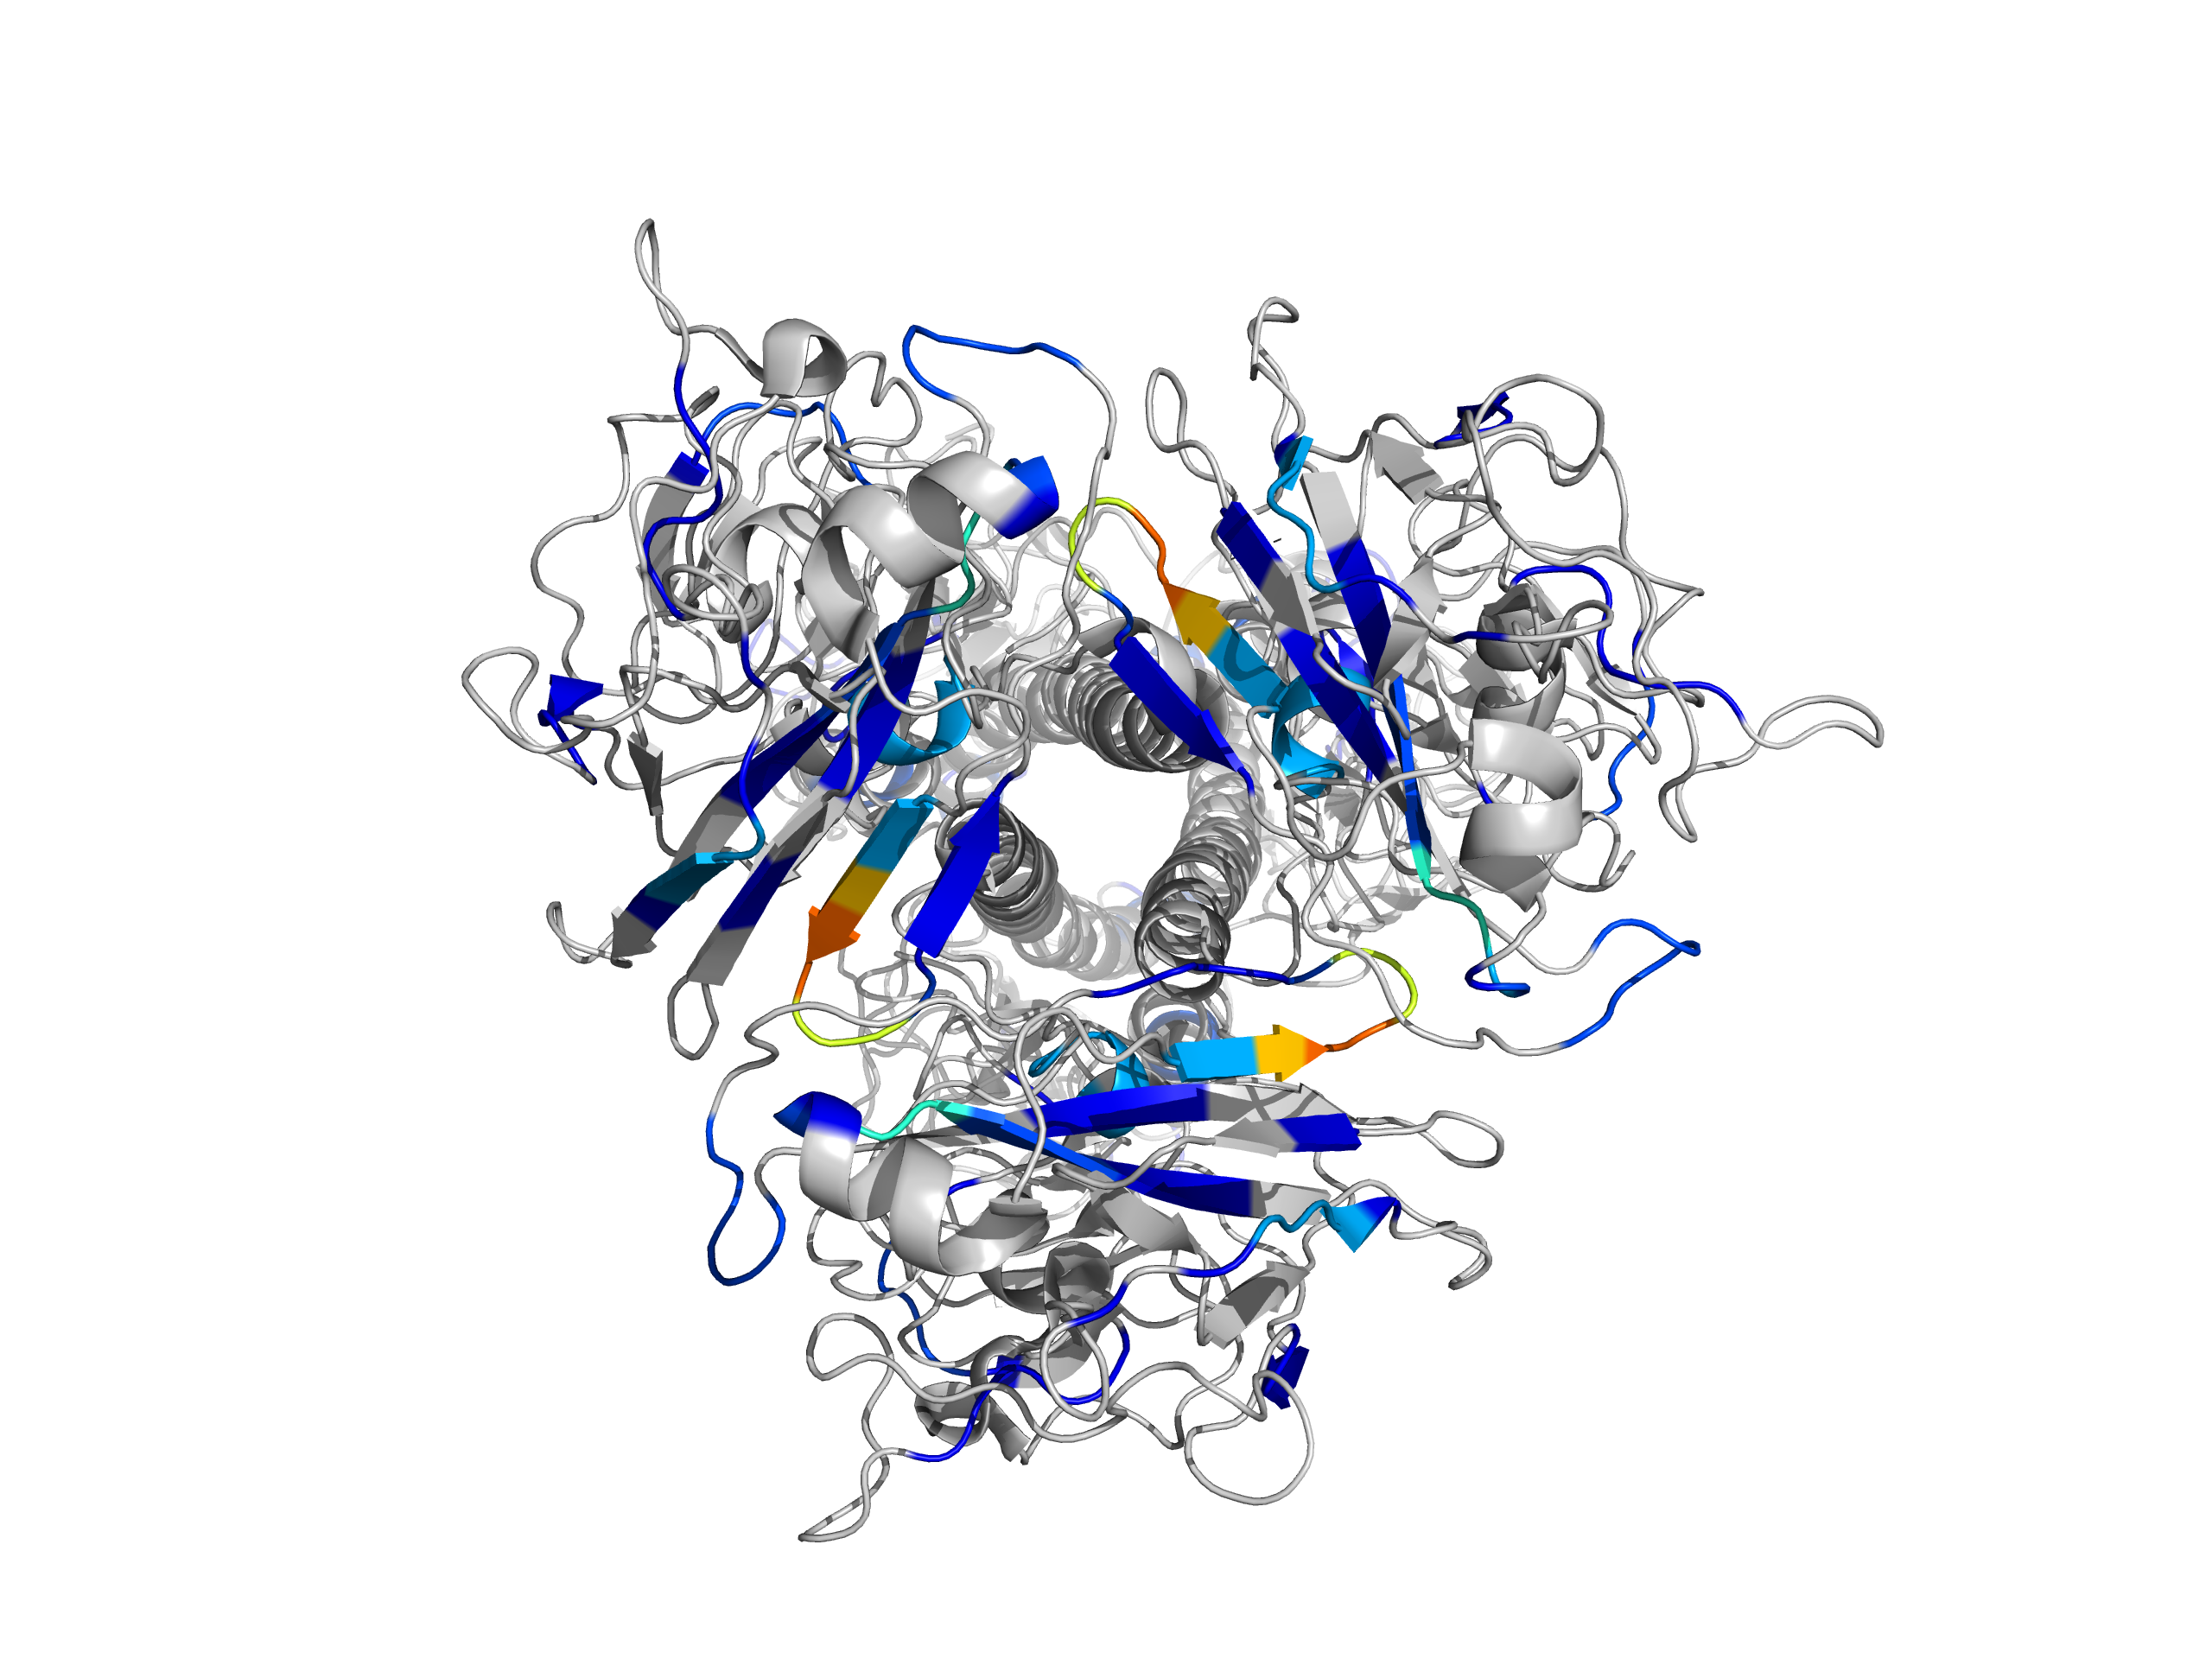
\includegraphics[width=2.75in]{/home/ishanu/ZED/Research/publications/pub_pan_one_/Figures/plotdata/seqanal/ntb/jetrndfile1.png}};
%  \node[anchor=north west] (T111) at ([yshift=-0.15in,xshift=0.05in]T11.south west) {
% 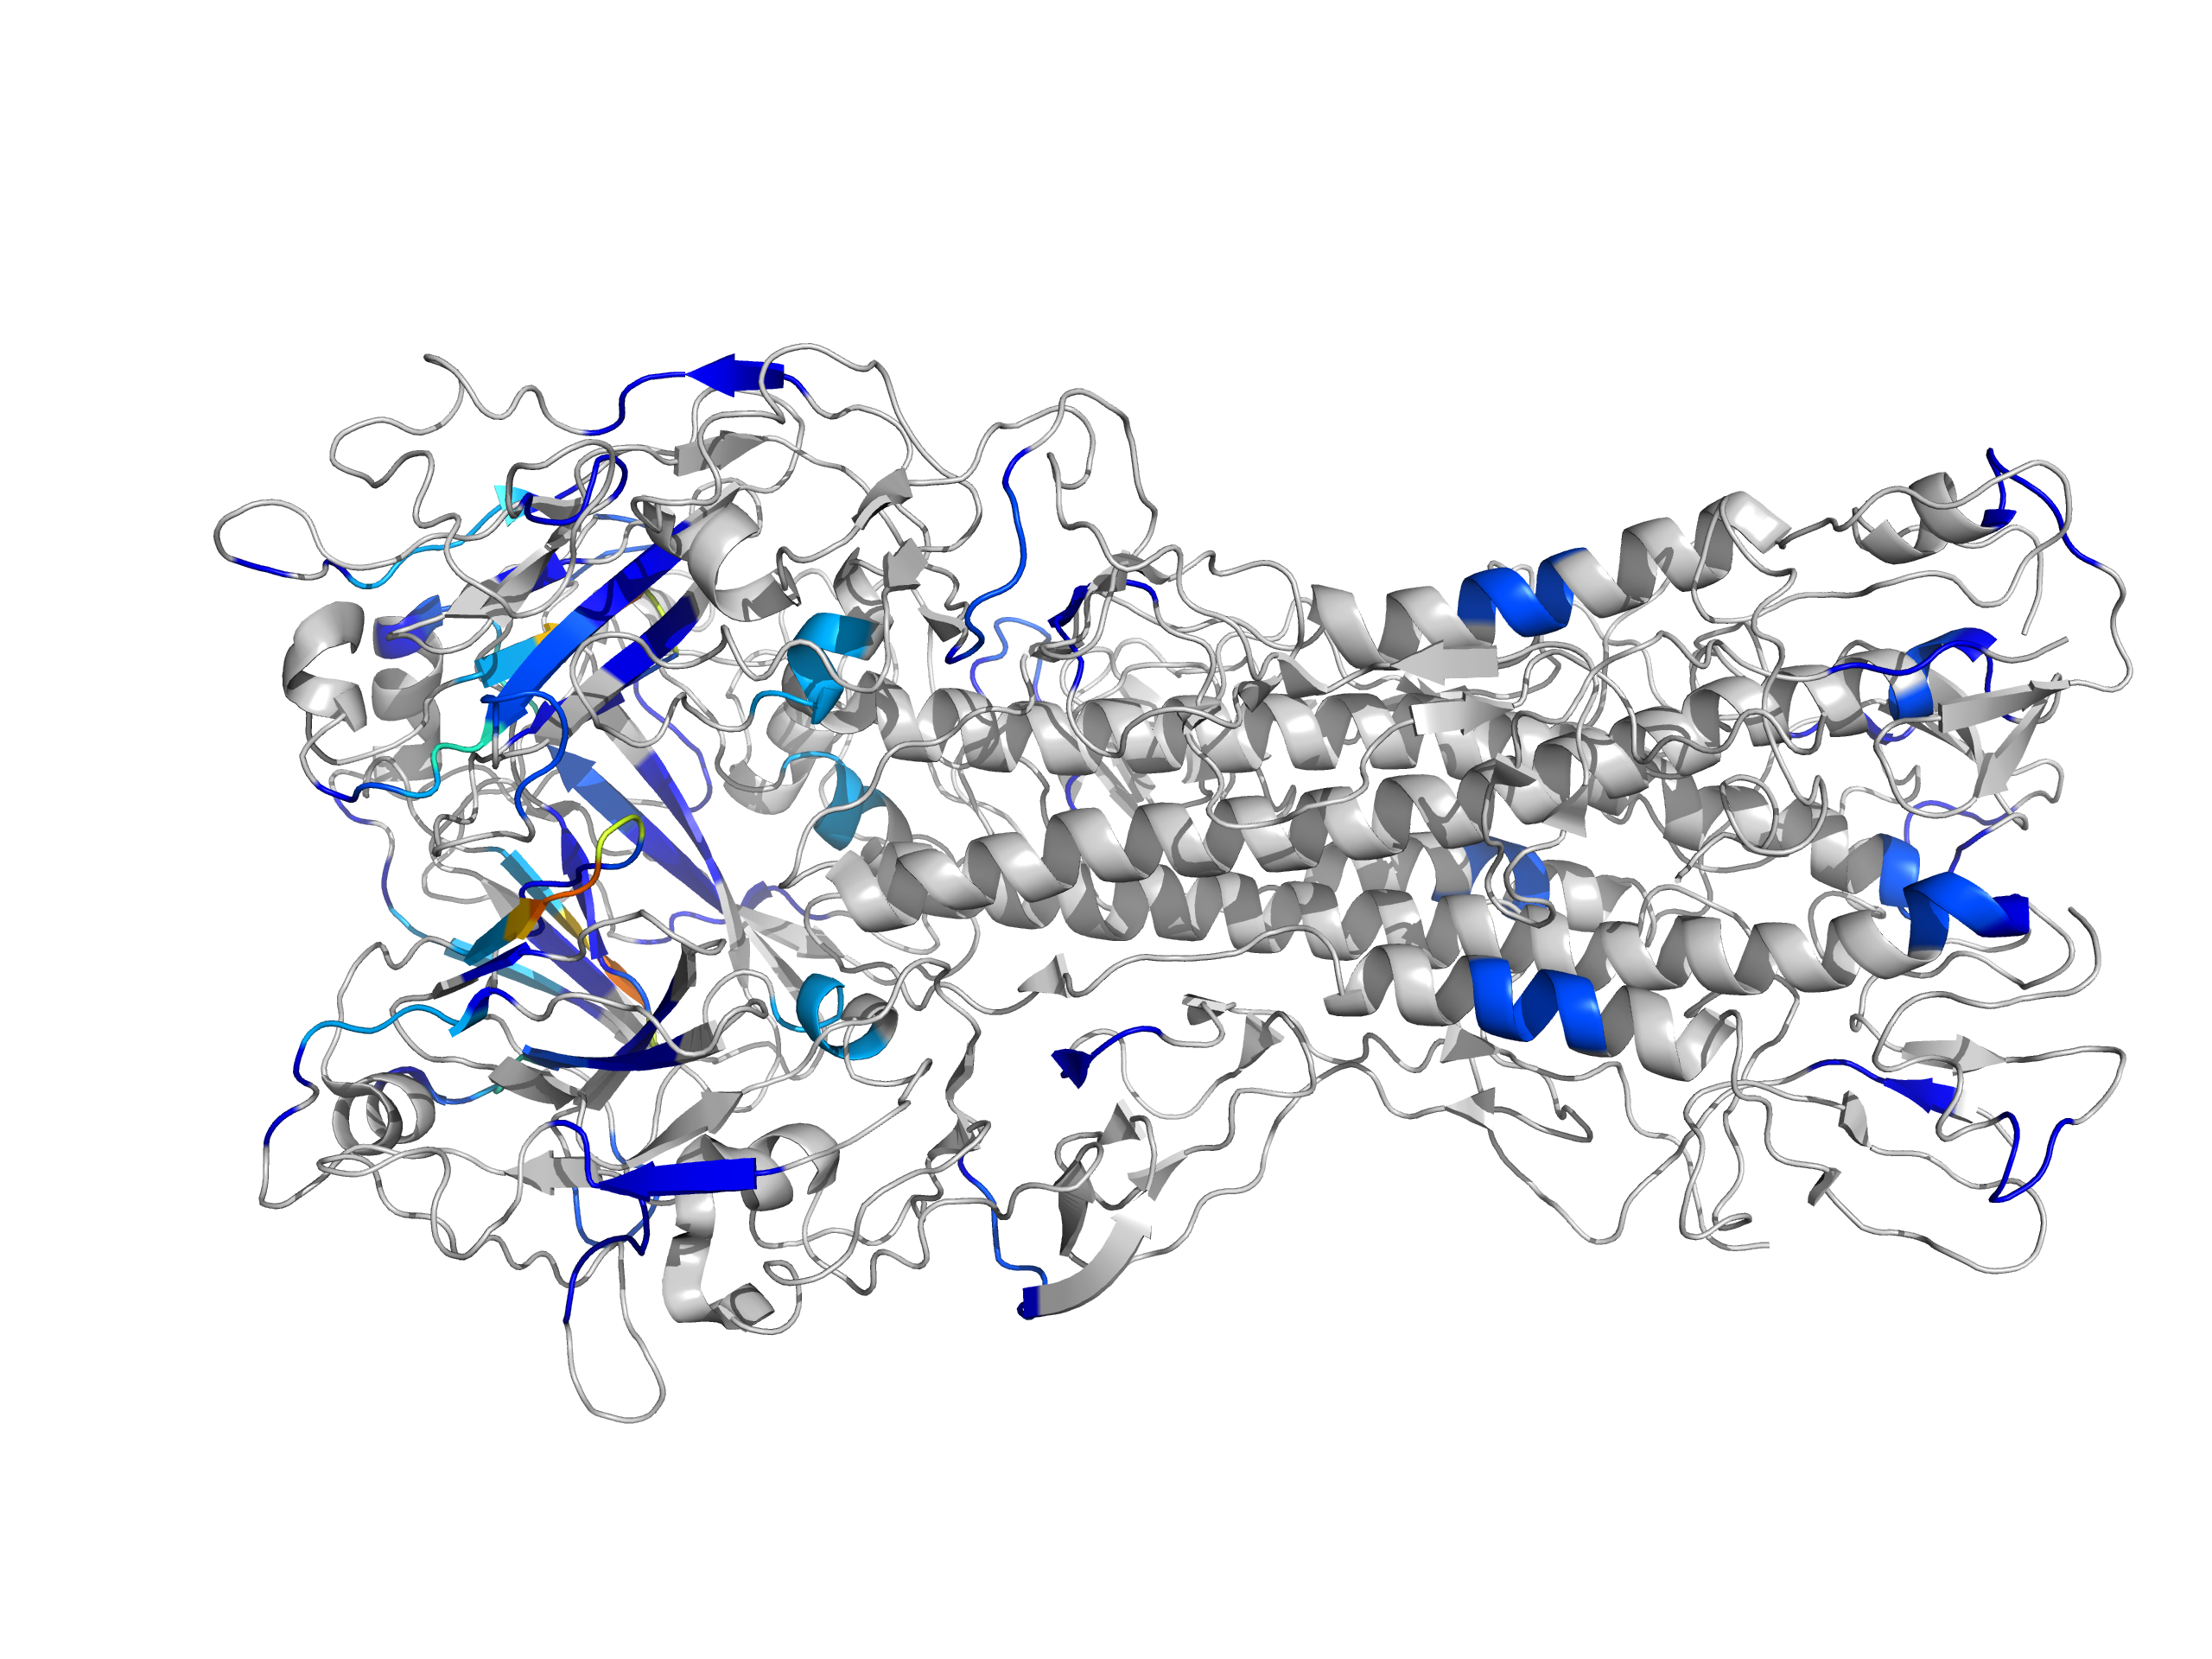
\includegraphics[width=3.5in,angle=-90]{/home/ishanu/ZED/Research/publications/pub_pan_one_/Figures/plotdata/seqanal/ntb/jetrndfile2.png}};
%  \node[anchor=north west] (T112) at ([yshift=0.2in,xshift=.86in]T11.south west) {
% 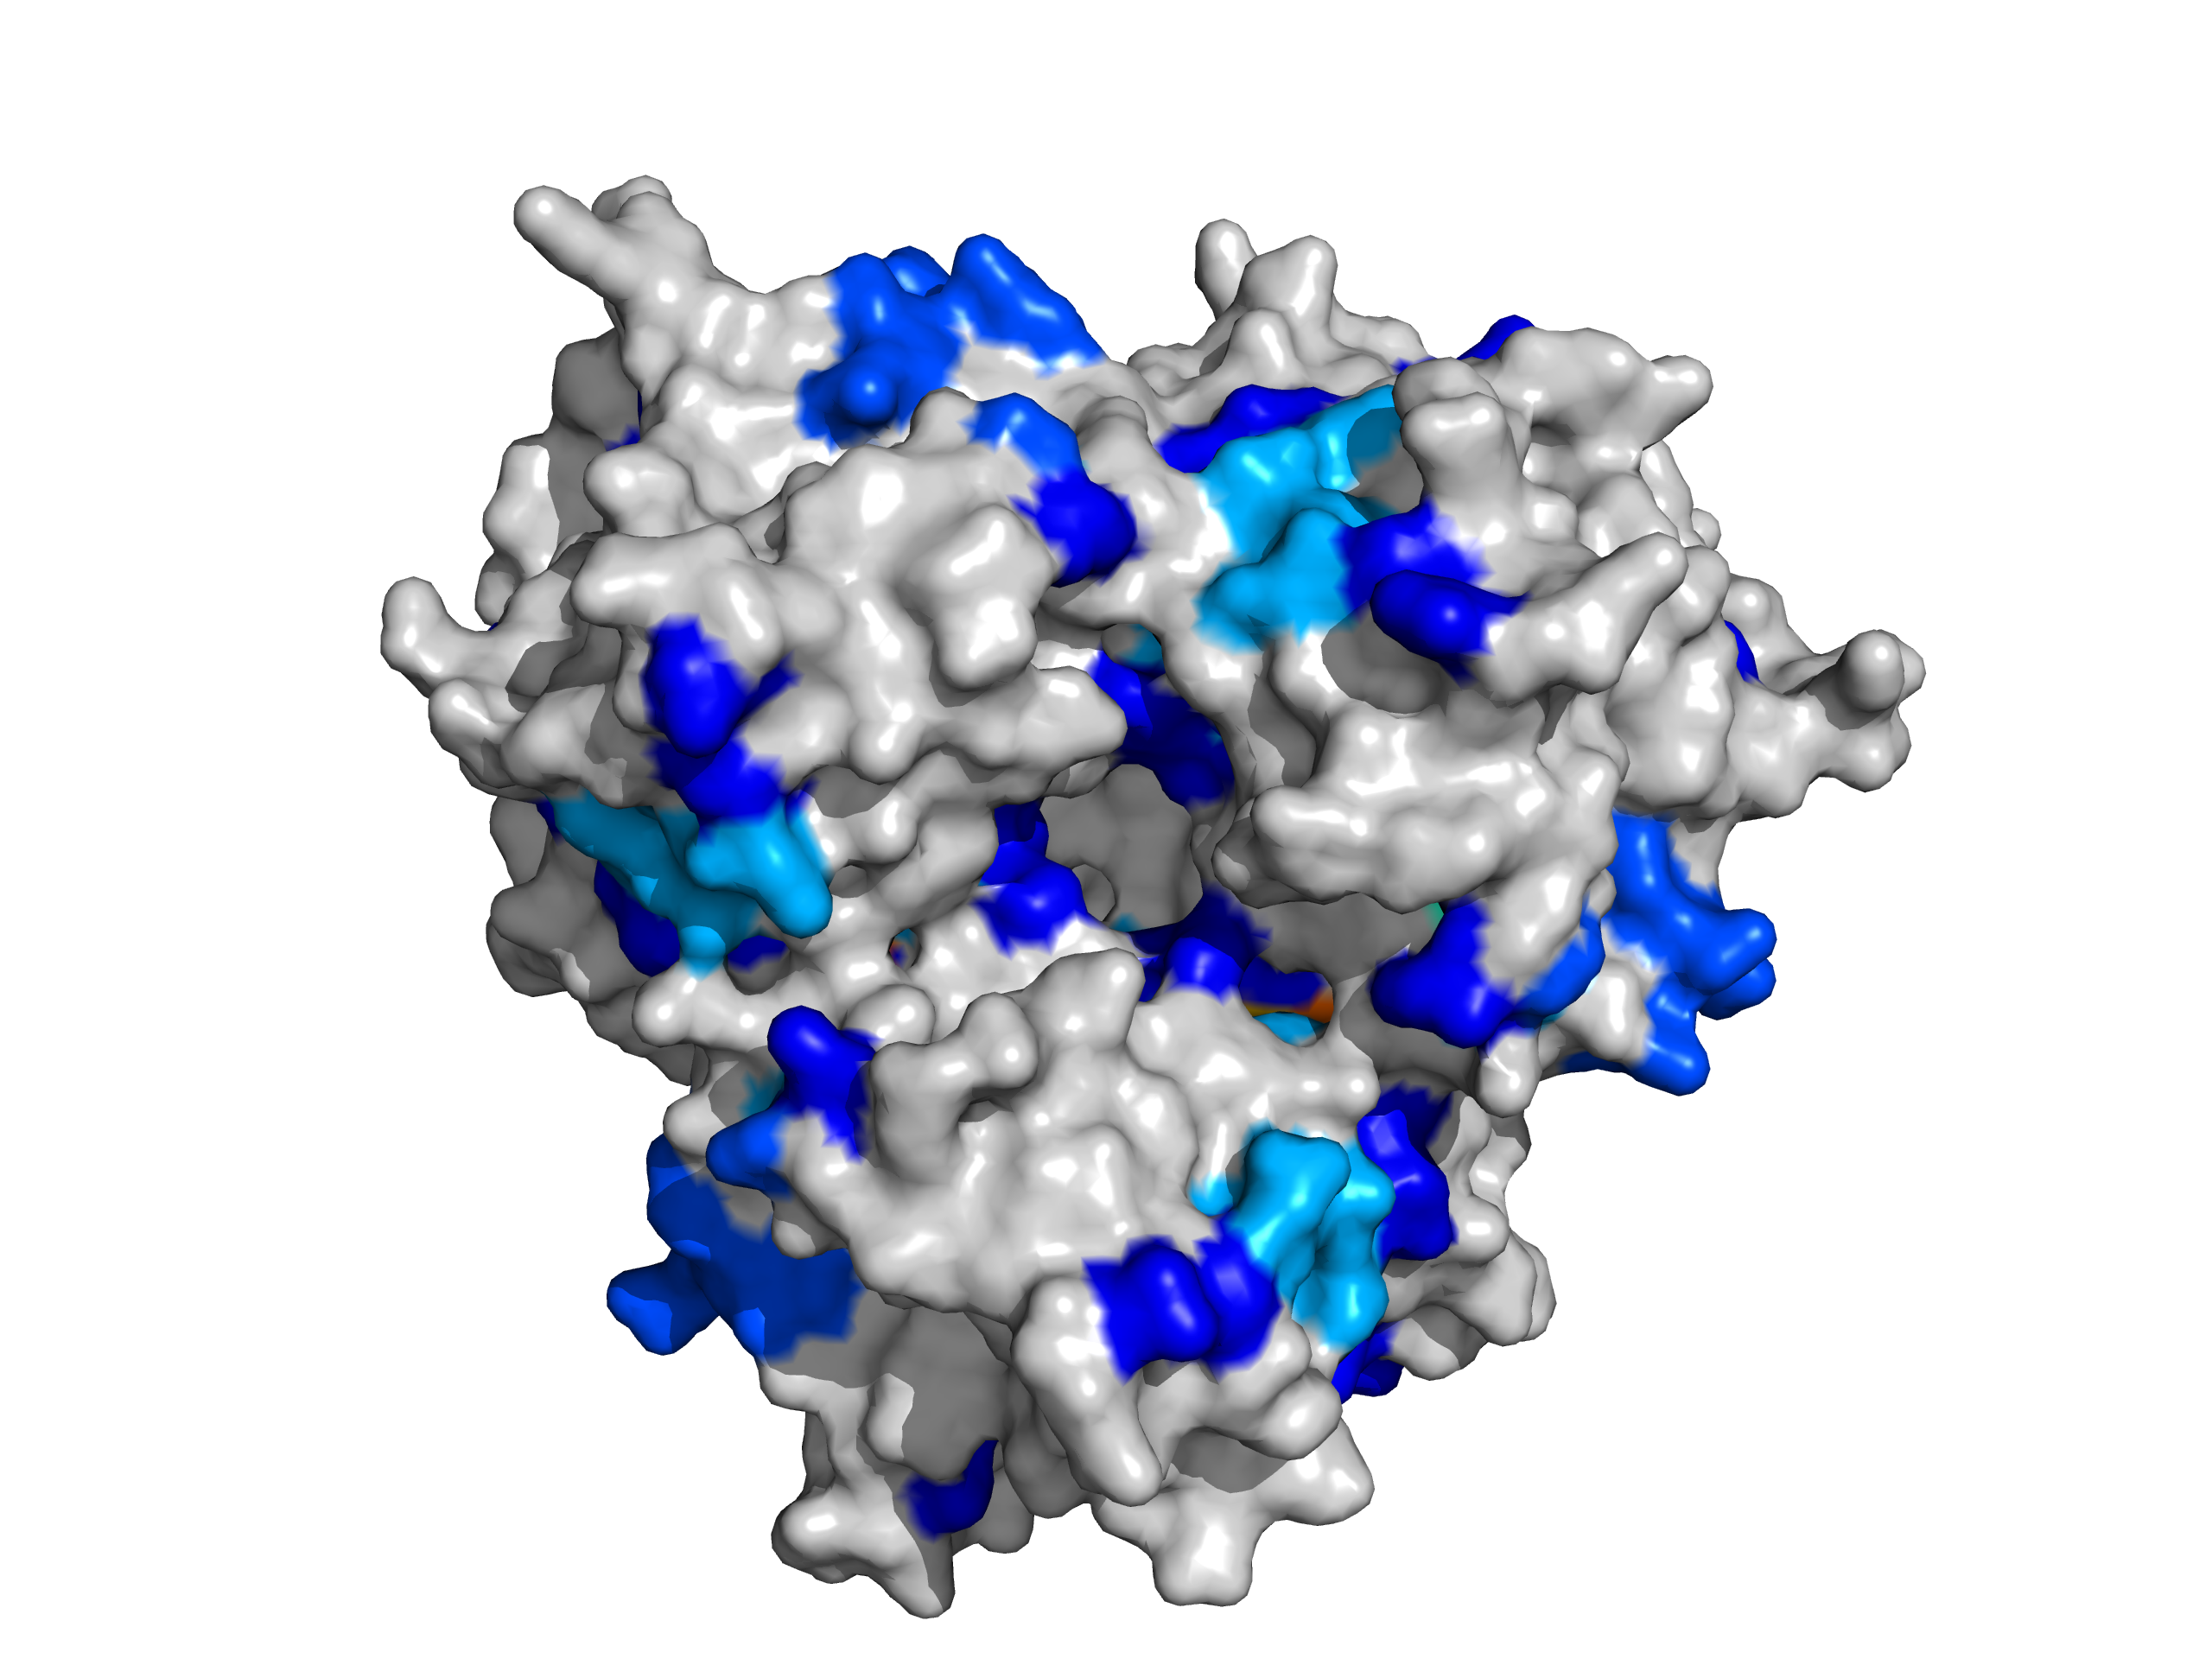
\includegraphics[width=1in]{/home/ishanu/ZED/Research/publications/pub_pan_one_/Figures/plotdata/seqanal/ntb/jetrndfile4.png}};
   

%  \node[anchor=north west] (L2) at ([xshift=.6in,yshift=-0.05in]$(T1.north west)!(T11.west)!(T1.north east)$) {{\large \normalfont g.}};
%  \node[anchor=north west] (L3) at ([xshift=.6in,yshift=-.1in]$(T11.north west)!(T112.north)!(T11.south west)$) {{\large \normalfont h.}};
%  \node[anchor=north west] (L4) at ([xshift=.6in,yshift=-.45in]$(T11.north west)!(T111.north)!(T11.south west)$) {{\large \normalfont i.}};

% \draw [thin, dashed] (T11.center) -- (T111.center);
% \draw [-{latex},thin,Red1] ([xshift=-.8in,yshift=-.5in]T11.center) -- ([xshift=-.38in,yshift=-.17in]T11.center) node [pos=0.1,xshift=-.15in,yshift=-.02in,font=\bf\sffamily\fontsize{6}{6}\selectfont,text=black] {200} ;
% \draw [-{latex},thin,Red1] ([xshift=-.8in,yshift=-.5in]T11.center) -- ([xshift=-0.12in,yshift=-2.1in]T11.center);
% \draw [-{latex},thin,Red1] ([xshift=.6in,yshift=-.65in]T11.center) -- ([xshift=.3in,yshift=-.29in]T11.center) node [pos=-0.15,font=\bf\sffamily\fontsize{6}{6}\selectfont,text=black,fill=white] {200};
% \draw [-{latex},thin,Red1] ([xshift=.1in,yshift=.7in]T11.center) -- ([xshift=.1in,yshift=.34in]T11.center) node [pos=-0.15,font=\bf\sffamily\fontsize{6}{6}\selectfont,text=black,fill=white] {200};

% \draw [-{latex},thin,Red1] ([xshift=.73in,yshift=-.45in]T11.center) -- ([xshift=.7in,yshift=-.2in]T11.center) node [pos=-0.15,font=\bf\sffamily\fontsize{6}{6}\selectfont,text=black,fill=white] {220};

% \draw [-{latex},thin,Red1] ([xshift=.73in,yshift=-.45in]T11.center) -- ([xshift=.7in,yshift=-.2in]T11.center) node [pos=-0.15,font=\bf\sffamily\fontsize{6}{6}\selectfont,text=black,fill=white] {220};

% \draw [-{latex},thin,Red1] ([xshift=.53in,yshift=-.35in]T11.center) -- ([xshift=.42in,yshift=-0.1in]T11.center) node [pos=-0.15,font=\bf\sffamily\fontsize{6}{6}\selectfont,text=black] {180};

% \draw [-{latex},thin,Red1] ([xshift=.53in,yshift=-.35in]T111.center) -- ([xshift=.42in,yshift=-0.6in]T111.center) node [pos=-0.15,xshift=.05in,font=\bf\sffamily\fontsize{6}{6}\selectfont,text=black] {49(HA2)};

% \draw [-{latex},thin,Red1] ([xshift=-.8in,yshift=-.15in]T111.center) -- ([xshift=-.35in,yshift=0.4in]T111.center) node [pos=-0.15,xshift=.05in,font=\bf\sffamily\fontsize{6}{6}\selectfont,text=black] {100};

% \draw [-{latex},thin,Red1] ([xshift=-1in,yshift=.2in]T111.center) -- ([xshift=-.6in,yshift=0.65in]T111.center) node [pos=-0.15,xshift=.05in,font=\bf\sffamily\fontsize{6}{6}\selectfont,text=black] {115};

% \draw [-{latex},thin,Red1] ([xshift=-.8in,yshift=-1.1in]T111.center) -- ([xshift=-0.1in,yshift=-1.32in]T111.center) node [pos=-0.15,xshift=.05in,yshift=.01in,font=\bf\sffamily\fontsize{6}{6}\selectfont,text=black] {124 (HA2)};


  
\end{tikzpicture}
 \else
  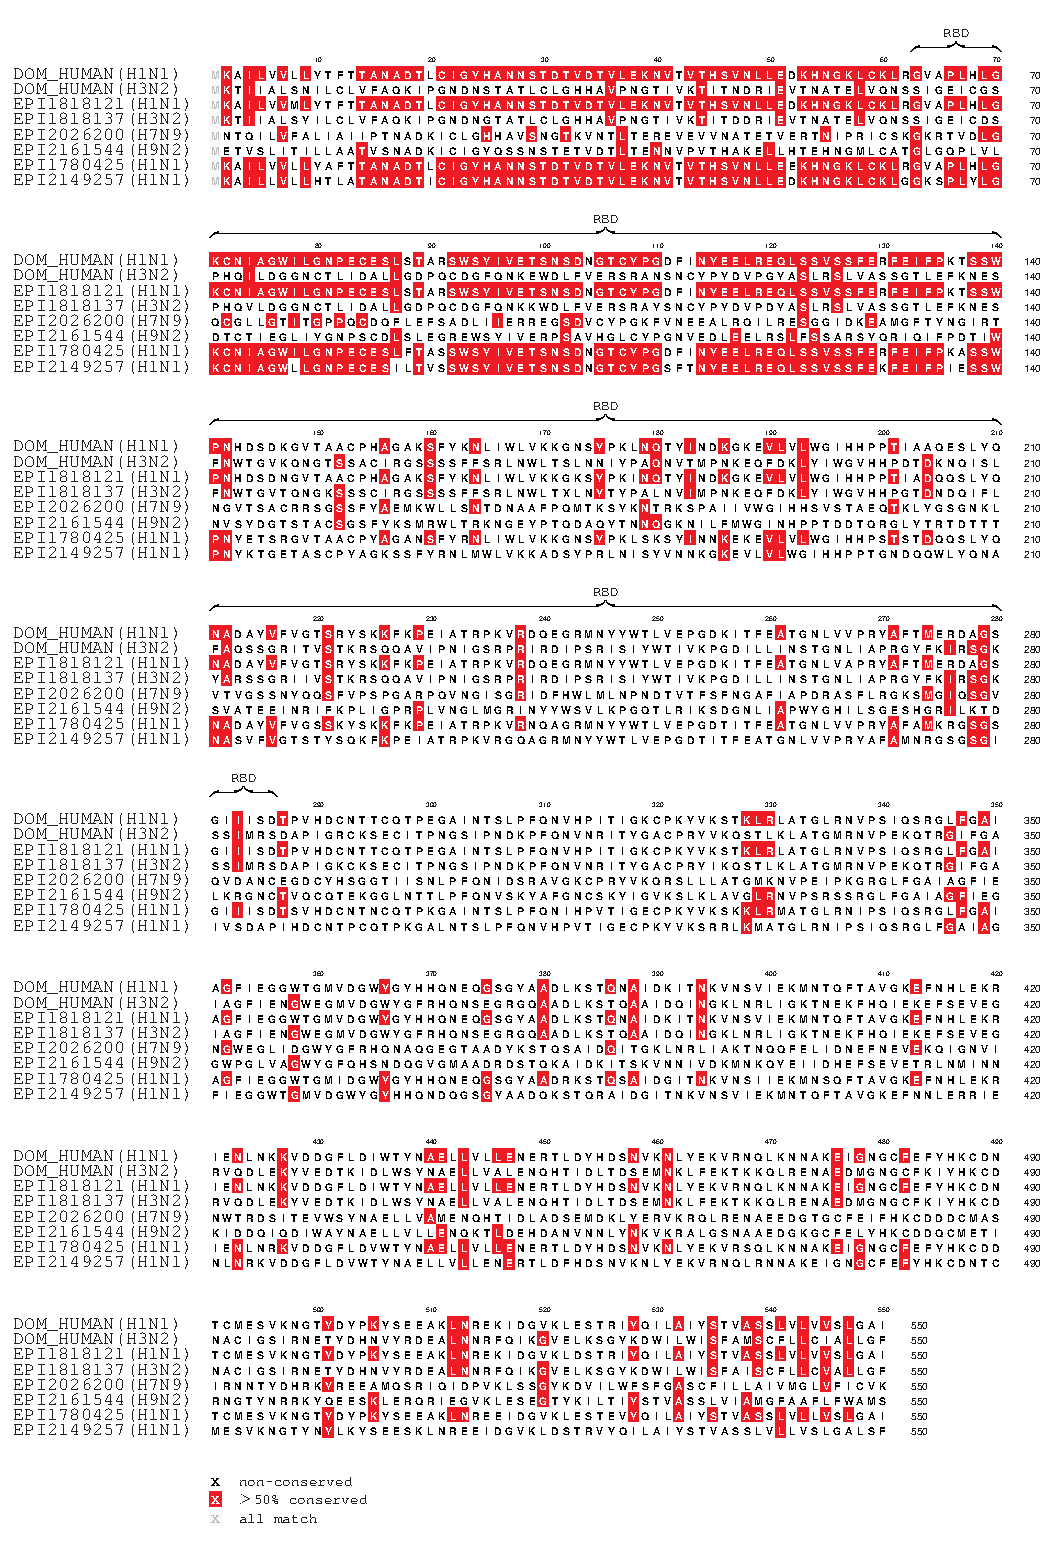
\includegraphics[width=.95\textwidth]{Figures/External/riskyseq}
  \fi 
  \vspace{-18pt}
  
\captionN{HA sequence comparison  with dominant human strains (DOM\_HUMAN H1N1, H3N2)  with \enet estimated top 5 risky strains (2020-2022 April) along with the teh most risky H9N2 strain (A/mink/China/chick embryo/2020), showing substantial differences from the circulating strains both in and out of the RBD. }\label{figriskyseq}
\end{figure}
\else
\refstepcounter{figure}\label{figriskyseq}
\fi

% #############################################

